% ITU Thesis/Dissertation
% Please see http://ee.tamu.edu/~tex for information about EE Thesis.

\documentclass[a4paper]{aitthesis}

\usepackage[utf8]{inputenc}
\usepackage[T1]{fontenc}
\usepackage{graphicx}
\usepackage{latexsym}
\usepackage{amssymb,amsthm,amsmath}
\usepackage{mathtools}
%\usepackage[notocbib]{apacite}
\usepackage{verbatim}
\usepackage{multirow}
\usepackage{bm}
\usepackage{url}
\usepackage{algorithm}
\usepackage{algcompatible}
\usepackage{placeins}
\usepackage{times}
\usepackage{array}
\usepackage[caption=false,font=footnotesize]{subfig}
\usepackage{tikz}
\usetikzlibrary{positioning, arrows.meta, shapes.geometric, calc, fit, backgrounds}
%\usepackage{setspace}
%\begin{onehalfspacing}
 % This paragraph has \\ double \\ line spacing.
%\end{onehalfspacing}

\newcommand{\oops}[1]{\bf{#1}}
\newcommand{\ga}{\bar{\gamma}}
\newcommand{\myint}{\int_0^{\infty}}
\renewcommand{\vec}[1]{\mathbf{#1}}
\newcommand{\mat}[1]{\mathrm{#1}}

\newcommand{\vectornorm}[1]{\left|\left|#1\right|\right|}

\newcommand{\ten}[1]{\mathcal{#1}}
\newcommand{\crossmat}[1]{\begin{bmatrix} #1 \end{bmatrix}_{\times}}
\newcommand{\class}[1]{{\cal C}_{#1}}
\def\Rset{\mathbb{R}}
\def\Pset{\mathbb{P}}
\DeclareMathOperator*{\argmax}{argmax}
\DeclareMathOperator*{\argmin}{argmin}
\DeclareMathOperator*{\sign}{sign}
\def\norm{\mbox{$\cal{N}$}}

\newcommand\parms{\vec{\lambda}}
\newcommand\oldparms{\parms^{\text{old}}}
%\renewcommand{\baselinestretch}{1.5} %for line spacing 1.5
\linespread{1.3} % 1.3 for one and half line spacing, 1.6 for double. https://en.wikibooks.org/wiki/LaTeX/Text_Formatting#Line_Spacing
\def\short{1}

\begin{document}

\pagenumbering{roman}
\pagestyle{plain}
%==========================================================
%======================  FRONT STUFF ======================
%==========================================================

%======================= Cover Page =======================
%\begin{document}
\newpage
\pagestyle{plain}
\pagenumbering{roman}
\setcounter{page}{5} %start of the page numbering, initial 4 pages are to be from Word document
\addcontentsline{toc}{section}{Title Page}
%\setlength{\footskip}{-15mm}
\setlength{\textheight}{230mm}
\setlength{\voffset}{10mm}
\vskip -5em

\begin{center}
{
  \singlespace \uppercase{\bf KinecMamba: Anatomy-Aware 3D Human Pose Estimation using Mamba} \par
}
\vskip 2em
{
  \lineskip 1.5em
  \begin{tabular}[t]{c} by\\ \\ Umar Rafaqat\\[0.3em] Student ID: MSDS24068
  \end{tabular}\par
}
\vskip 5.6em

\vskip 3.5em
\singlespace A thesis submitted in partial fulfillment of the
requirements for the\\ degree of Master of Science in\\
Data Science % verify: degree/program

	\vskip 5em
\vskip 0.5em
{
  \singlespace
 \begin{center}
   \begin{tabular}{rl}
     \\[-1em]
    Supervisor: & Dr.\ Mehwish Ghafoor \\[-0.8em]
                & \\[-0.8em]
    Examination Committee: & Dr.\ [PLACEHOLDER: Committee Member \#1] \\[-0.8em]
                           & Dr.\ [PLACEHOLDER: Committee Member \#2] \\\\
   \end{tabular}
 \end{center}

 \vskip 3.0em
  \centerline{}
 \vskip 2em
}
\end{center}
\begin{center}
  \singlespace Information Technology University (ITU), Lahore\\ % verify institution
  Month Year % verify submission date
\end{center}
\vfill

%====================== DECLARATION ======================
\newpage
\pagestyle{plain}
\addcontentsline{toc}{section}{Declaration}
\begin{center}
{\large \bf Declaration\\ \vskip 1em}
\end{center}
\singlespace
\vspace{1em}

\noindent I, Umar Rafaqat (Student ID: MSDS24068), declare that this thesis titled
``KinecMamba: Anatomy-Aware 3D Human Pose Estimation using Mamba'' and the work
presented in it are my own. This work was carried out under the supervision of
Dr.\ Mehwish Ghafoor at Information Technology University (ITU), Lahore. Where I have
drawn on the work of others, it has been cited and acknowledged. This thesis has not
been submitted for any other degree.

\vskip 4em
\noindent Signature: \underline{\hspace{5cm}} \hfill Date: \underline{\hspace{3.5cm}}

%====================== ACKNOWLEDGEMENTS ======================
\newpage
\pagestyle{plain}
\addcontentsline{toc}{section}{Acknowledgments}
\onecolumn % Single-column.
\if@twoside\else\raggedbottom\fi % Ragged bottom unless twoside option.
\setlength{\footskip}{8mm}
\begin{center}
{
  \large \bf Acknowledgments\\ \vskip 1em
}
\vskip 1em
\end{center}
\singlespace
\doublespace
\hspace{8.5mm}
\vspace{-1em}

\noindent I am grateful to my supervisor, Dr.\ Mehwish Ghafoor, for her guidance and
support throughout this work. I thank the faculty of Information Technology University
(ITU), Lahore for the resources and environment that made this research possible, and
my family and colleagues for their encouragement.

%======================= Table of Contents =========================
\newpage
\addcontentsline{toc}{section}{Table of Contents}
\tableofcontents

% Page 2 begins

%===================== List of Figures ======================
\newpage
\addcontentsline{toc}{section}{List of Figures}
\listoffigures

%\clearpage     % \clearpage ends the page, and also dumps out all floats.
%\end{document} % Floats are things like tables and figures.

%\clearpage     % \clearpage ends the page, and also dumps out all floats.

% %===================== List of Tables ======================
\newpage
\addcontentsline{toc}{section}{List of Tables}
\listoftables

% %\clearpage     % \clearpage ends the page, and also dumps out all floats.
% %\end{document} % Floats are things like tables and figures.

%\clearpage     % \clearpage ends the page, and also dumps out all floats.
\setlength{\parskip}{12pt}

%====================== ABSTRACT ======================
\newpage
\pagestyle{plain}
\addcontentsline{toc}{section}{Abstract}
\onecolumn % Single-column.
\if@twoside\else\raggedbottom\fi % Ragged bottom unless twoside option.

\setlength{\footskip}{8mm}

\begin{center}
{\large \bf Abstract \\ \vskip 1em}
\vskip 1em
\end{center}
\singlespace
\doublespace
\hspace{8.5mm}
\vspace{-1em}

Monocular 3D human pose estimation recovers the three-dimensional positions of body
joints from single-camera video. The task is usually solved in two stages: a 2D
detector locates joints on the image, and a lifting network maps the resulting 2D
keypoint sequence to 3D. Transformer-based lifting networks model spatial and
temporal dependencies well, but their self-attention scales quadratically with the
number of spatio-temporal tokens, which caps the temporal context they can afford.
State space models such as Mamba reach comparable modelling quality at linear cost,
yet they read their input as a single ordered sequence, while a human skeleton has no
natural order. Feeding the joints in raw index order places anatomically distant
joints next to each other and weakens the model's grasp of local structure. This
thesis presents KinecMamba, a bidirectional spatio-temporal state space network for
2D-to-3D pose lifting. It preserves the linear cost of Mamba through a
four-directional cross-scan over the frame and joint axes, and orders the joints
along the spatial scan by a breadth-first traversal of the skeleton's kinematic tree,
from the pelvis outward along each limb. An anatomy-aware bone-length loss supervises
the lengths and temporal consistency of the skeleton's bones, reinforcing the same
structure the scan follows. KinecMamba is evaluated on Human3.6M and MPI-INF-3DHP
against Transformer- and state-space-based methods, with an ablation that isolates the
scan order from the rest of the network.

\setlength{\parskip}{0pt}



\small

\pagenumbering{arabic}
\setlength{\headheight}{12pt}
\pagestyle{plain}

\setlength{\footskip}{8mm}

\chapter{Introduction}
\label{ch:introduction}

\section{Overview}
\label{sec:intro-overview}

Human pose estimation from monocular video supports a wide range of
applications, including motion capture for animation, human-computer
interaction, sports performance analysis, surveillance, and autonomous
driving \cite{guo2025survey3dhpe}. Among the various formulations of this
problem, monocular 3D human pose estimation (HPE), which recovers the
three-dimensional coordinates of human body joints from a single-camera
video sequence, remains particularly challenging, since a single 2D
projection is inherently ambiguous with respect to depth. The dominant
paradigm decomposes the task into two stages: a 2D pose detector localizes
keypoints on the image plane, after which a 2D-to-3D lifting network infers
the corresponding 3D joint positions from the resulting 2D keypoint
sequence \cite{pavllo2019videopose3d}. Depth ambiguity and self-occlusion
make this second stage, lifting, the central technical difficulty the
field has focused on for the past decade.

Early lifting approaches relied on convolutional architectures.
Representative work such as HRNet \cite{sun2019hrnet} demonstrated that
maintaining high-resolution feature representations throughout the network
improves keypoint localization accuracy, but convolutional
receptive fields remain inherently local, limiting these models' ability
to reason jointly across distant body parts and across long temporal
windows. The introduction of the Transformer architecture
\cite{vaswani2017attention} and its extension to vision
\cite{dosovitskiy2020vit} offered a remedy: self-attention allows every
joint, at every frame, to directly attend to every other joint and frame.
PoseFormer \cite{zheng2021poseformer} was the first to apply spatial and
temporal self-attention to 3D HPE, and subsequent work refined this idea
along several axes. MHFormer \cite{li2022mhformer} models multiple
plausible pose hypotheses to resolve depth ambiguity, MixSTE
\cite{zhang2022mixste} alternates spatial and temporal transformer blocks
in a sequence-to-sequence formulation, PoseFormerV2
\cite{zhao2023poseformerv2} exploits the frequency domain to reduce
sequence length, STCFormer \cite{tang2023stcformer} models spatial and
temporal correlations jointly through criss-cross attention, and
MotionBERT \cite{zhu2023motionbert} and MotionAGFormer
\cite{mehraban2024motionagformer} pursue unified motion representations
and hybrid Transformer-GCN designs, respectively. However, the
self-attention mechanism these methods rely on incurs quadratic
computational and memory complexity in sequence length, and processes
spatio-temporal correlations in a manner that does not naturally
distinguish the directionality or hierarchy inherent to human skeletal
structure. As the field pushes toward longer input sequences for more
temporally consistent predictions, this quadratic cost becomes an
increasingly severe practical bottleneck.

The open question is whether a sequence model can capture the same
long-range spatio-temporal dependencies that make Transformers effective
for 3D HPE while scaling linearly rather than quadratically with sequence
length. Structured state space models (SSMs) have recently emerged as a
candidate answer. The S4 model \cite{gu2021s4} demonstrated that a
structured, continuous-time state space formulation can model long
sequences efficiently, and Mamba \cite{gu2023mamba} extended this line of
work with input-dependent (selective) parameterization and a
hardware-aware scan algorithm, achieving Transformer-competitive quality
with linear-time complexity. This efficiency prompted rapid adoption in
vision: Vision Mamba \cite{zhu2024visionmamba} and VMamba
\cite{liu2024vmamba} adapted the originally causal, unidirectional SSM
formulation to non-causal 2D visual data through bidirectional and
multi-directional scanning strategies, and SSMs have since been applied to
human motion and pose estimation directly
\cite{mondal2024hummuss, zhang2024posemagic, nguyen2025skeletonmamba,
zheng2025mambatopology, lu2025structureawaremamba, feng2025highresssm,
cui2025sasmamba, wang2025dbmambapose}.

Across this emerging body of work, a plain unidirectional SSM applied
naively to skeletal data tends to underperform, and some form of
bidirectional processing or custom scan ordering is needed to compensate
for the fact that an SSM processes its input as a
strict 1D sequence, whereas a human skeleton is not linear but a
hierarchical, tree-structured graph of joints connected by bones
\cite{yan2018stgcn, loper2015smpl}. Existing remedies to this mismatch are
largely heuristic or learned: some methods reorder joints according to an
ad hoc geometric heuristic, while others, such as the Group Scan and Joint
Scan strategies explored in \cite{nguyen2025skeletonmamba}, learn scan
groupings directly from data. Yet the general finding that a principled,
deterministic node ordering can markedly improve sequential modeling of
graph-structured data is well established outside the pose estimation
literature. Breadth-first search (BFS) ordering, for instance, has been
shown to make auto-regressive sequence models over graphs both more
scalable and more effective by exposing local graph structure to the
sequence model in a consistent, canonical way \cite{you2018graphrnn}. This
suggests that the skeleton's own kinematic tree, rather than a learned or
arbitrary heuristic, may offer a more principled scan order for SSM-based
pose estimation.

In this thesis, we investigate this direction directly. We adopt a
bidirectional spatio-temporal state space architecture for monocular 3D
human pose estimation, and introduce a breadth-first search (BFS)
kinematic-tree scan as an architectural refinement to the spatial scan
order: joints are traversed outward from a root joint (the pelvis)
following the parent-child hierarchy defined by the body's kinematic tree
\cite{loper2015smpl}, layer by layer, before being flattened into the 1D
sequence consumed by the state space model. This is motivated by the
hypothesis that a scan order derived directly from skeletal anatomy,
rather than from a fixed joint index or a learned grouping, better
preserves local joint adjacency for the SSM's local modeling capacity
while remaining simple, deterministic, and free of additional learned
parameters. We evaluate this approach on the standard Human3.6M
\cite{ionescu2014human36m} and MPI-INF-3DHP \cite{mehta2017mpiinf3dhp}
benchmarks against established Transformer-, GCN-, and SSM-based
baselines.

\section{Problem Statement}
\label{sec:intro-problem-statement}

The literature reviewed in Section~\ref{sec:intro-overview}
reveals two distinct, compounding problems that motivate the architecture
developed in this thesis.

\textbf{Problem 1: the computational cost of attention-based
spatio-temporal modeling.} Transformer-based 3D HPE methods
\cite{zheng2021poseformer, li2022mhformer, zhang2022mixste,
zhao2023poseformerv2, tang2023stcformer, zhu2023motionbert,
mehraban2024motionagformer} rely on self-attention to model relationships
across joints and frames, but self-attention's computational and memory
cost scales quadratically with input sequence length. Since prediction
accuracy in 3D HPE benefits from longer temporal context (more frames
give the model more evidence to disambiguate depth and resolve occlusion),
this quadratic scaling directly limits how much temporal context these
models can practically exploit, and forces a trade-off between temporal
receptive field and computational budget that becomes increasingly costly
as sequence length grows.

\textbf{Problem 2: a mismatch between sequential state space modeling and
the skeleton's non-sequential structure.} State space models such as
Mamba \cite{gu2023mamba} process input as a strict one-dimensional
sequence, and were originally formulated for inherently sequential or
unidirectional data. A human skeleton, however, is not a sequence but a
hierarchical, tree-structured graph of joints connected by rigid bones
\cite{loper2015smpl}, with no canonical linear order. Flattening this
graph into a 1D sequence therefore requires an explicit choice of scan
order, and this choice determines which joints appear adjacent to one
another in the sequence the SSM processes, which directly affects the
model's ability to capture local joint dependencies. Existing approaches
to this problem are unsatisfying in one of two ways: they either impose a
fixed but anatomically arbitrary order (e.g., dataset joint-index order,
or a hand-designed geometric heuristic), or they learn a scan grouping
from data, such as the Group Scan and Joint Scan strategies in
\cite{nguyen2025skeletonmamba}, at the cost of additional learned
parameters and reduced interpretability. Neither approach derives the scan
order directly and deterministically from the skeleton's own kinematic
hierarchy, despite evidence from outside the pose estimation literature
that principled graph-node orderings, such as breadth-first search, can
markedly improve sequential models over graph-structured data
\cite{you2018graphrnn}.

These two problems together define the central question this
thesis addresses: \textbf{how can a sequence model be designed that
retains the linear-time efficiency of state space models while processing
the human skeleton in a manner that respects its underlying kinematic
structure, rather than an arbitrary or learned joint ordering?} The
remainder of this thesis develops and evaluates an architecture that
answers this question through a bidirectional spatio-temporal state space
backbone combined with a deterministic, breadth-first search
kinematic-tree scan order.

\section{Objectives}
\label{sec:intro-objectives}

Guided by the problem statement in Section~\ref{sec:intro-problem-statement},
the objectives of this thesis are as follows:

\begin{enumerate}
  \item \textbf{To design a bidirectional spatio-temporal state space
    architecture for monocular 3D human pose estimation} that models both
    intra-frame joint relationships and inter-frame temporal correlations
    while retaining the linear-time computational complexity of state
    space models \cite{gu2023mamba, gu2021s4}, avoiding the quadratic
    scaling of self-attention-based approaches \cite{zheng2021poseformer,
    zhang2022mixste, zhu2023motionbert}.

  \item \textbf{To introduce a breadth-first search (BFS) kinematic-tree
    scan order} as the spatial scan strategy for this architecture,
    traversing the skeleton's joints outward from a root joint according
    to the parent-child hierarchy defined by the body's kinematic tree
    \cite{loper2015smpl}, as a deterministic, anatomically-grounded
    alternative to the fixed-index and learned scan orders used in prior
    SSM-based pose estimation work \cite{nguyen2025skeletonmamba},
    motivated by evidence that BFS node orderings improve sequential
    modeling of graph-structured data \cite{you2018graphrnn}.

  \item \textbf{To empirically evaluate the proposed architecture} on the
    standard Human3.6M \cite{ionescu2014human36m} and MPI-INF-3DHP
    \cite{mehta2017mpiinf3dhp} benchmarks, comparing accuracy (MPJPE) and
    computational efficiency (parameter count, MACs) against
    representative Transformer-based \cite{zhang2022mixste,
    zhu2023motionbert, mehraban2024motionagformer}, graph-based
    \cite{yu2023glagcn}, and state-space-based \cite{zhang2024posemagic,
    cui2025sasmamba, wang2025dbmambapose} baselines.

  \item \textbf{To isolate and quantify the specific contribution of the
    BFS kinematic-tree scan} through ablation studies comparing it against
    alternative scan orders (e.g., fixed joint-index order, learned
    group/joint scan strategies), in order to determine whether any
    performance difference is attributable to the scan order itself rather
    than to the underlying SSM backbone alone.
\end{enumerate}

\section{Limitations and Scope}
\label{sec:intro-limitations}

This thesis focuses specifically on the 2D-to-3D lifting stage of the
monocular 3D human pose estimation pipeline. Several boundaries define the
scope of this work:

\begin{itemize}
  \item \textbf{Single-person, monocular RGB input.} The proposed
    architecture is designed and evaluated for single-person 3D pose
    estimation from a single RGB camera viewpoint. Multi-person scenarios,
    multi-view fusion, and depth-sensor or inertial-sensor inputs fall
    outside the scope of this thesis.

  \item \textbf{2D keypoint input assumed.} Consistent with the standard
    2D-to-3D lifting formulation \cite{pavllo2019videopose3d}, this thesis
    assumes 2D keypoints are available as input, either from ground-truth
    annotations or an off-the-shelf 2D pose detector \cite{sun2019hrnet}.
    Improving 2D keypoint detection accuracy itself is not an objective of
    this work; errors introduced at the 2D detection stage are treated as
    an external input condition rather than a problem this architecture
    addresses.

  \item \textbf{Evaluation limited to standard benchmark datasets.} The
    proposed method is evaluated on Human3.6M \cite{ionescu2014human36m}
    and MPI-INF-3DHP \cite{mehta2017mpiinf3dhp}, both of which are
    captured under controlled or semi-controlled conditions. Performance
    on fully unconstrained in-the-wild video, where ground-truth 3D
    annotations are unavailable for direct quantitative evaluation, is not
    assessed.

  \item \textbf{Fixed, known skeletal topology.} The breadth-first search
    kinematic-tree scan relies on a fixed, predefined parent-child joint
    hierarchy \cite{loper2015smpl} consistent with the skeletal
    definitions used by the evaluation datasets. This thesis does not
    address generalization to non-standard skeletal topologies (e.g.,
    pathological anatomy, partial-body input, or rigs with a different
    joint count/hierarchy) that would require re-deriving the traversal
    order.

  \item \textbf{Efficiency measured, not deployed.} Computational
    efficiency is assessed in terms of parameter count and
    multiply-accumulate operations (MACs), consistent with prior work
    \cite{zhang2024posemagic, cui2025sasmamba}. This thesis does not
    include on-device deployment, latency benchmarking on embedded or
    mobile hardware, or real-time system integration.

  \item \textbf{Architectural scope.} The contribution of this thesis is
    confined to the sequence backbone and spatial scan order of the
    lifting network. Improvements to loss functions, data augmentation
    strategies, temporal post-processing/smoothing, or multi-hypothesis
    modeling \cite{li2022mhformer} are outside the scope of this work,
    except where a standard, established choice is adopted without
    modification to support the core architectural comparison.
\end{itemize}

\section{Thesis Outline}
\label{sec:intro-outline}

The remainder of this thesis is organized as follows.

Chapter~\ref{ch:literature-review} reviews the literature relevant to this
work, tracing the evolution of monocular 3D human pose estimation from
convolutional and graph-based methods, through Transformer-based
architectures, to the recent emergence of state space models, and
situates the kinematic-tree scan order proposed in this thesis within that
context.

Chapter~\ref{ch:methodology} presents the proposed architecture in detail,
including the bidirectional spatio-temporal state space backbone and the
breadth-first search kinematic-tree scan.

Chapter~\ref{ch:results} reports the experimental setup and benchmark
results on Human3.6M and MPI-INF-3DHP, comparisons against Transformer-,
graph-, and state-space-based baselines, and ablation studies isolating
the effect of the proposed scan order.

Finally, Chapter~\ref{ch:conclusion} summarizes the contributions of this
thesis, discusses its limitations, and outlines directions for future
work.

\FloatBarrier


\setlength{\footskip}{8mm}

\chapter{Literature Review}
\label{ch:literature-review}

\section{Overview}
\label{sec:lit-overview}

This chapter surveys the literature underlying the architecture
developed in this thesis, organized to trace the field's evolution from
its earliest formulations to the specific research gap this work
addresses. Section~\ref{sec:lit-pipeline} establishes the two-stage
2D-to-3D lifting pipeline that frames the rest of the chapter.
Section~\ref{sec:lit-conv-graph} reviews convolutional and graph-based
lifting approaches, including early treatments of the human skeleton as a
graph. Section~\ref{sec:lit-transformer} traces the Transformer-based
lineage of 3D human pose estimation methods and the quadratic-complexity
limitation they share. Section~\ref{sec:lit-ssm-foundations} introduces
structured state space models and the Mamba architecture as a
linear-complexity alternative to self-attention.
Section~\ref{sec:lit-ssm-pose} reviews the emerging body of work applying
state space models to human motion and pose estimation directly.
Section~\ref{sec:lit-skeleton-ordering} examines how sequential models
represent and order graph-structured data such as the human skeleton,
drawing on evidence from outside the pose estimation literature. Finally,
Section~\ref{sec:lit-summary-gap} synthesizes this review into an explicit
statement of the research gap, connecting directly to the problem
statement in Section~\ref{sec:intro-problem-statement} and motivating the
architecture presented in Chapter~\ref{ch:methodology}.

\section{The Two-Stage 3D Human Pose Estimation Pipeline}
\label{sec:lit-pipeline}

The majority of monocular 3D human pose estimation methods, including the
architecture developed in this thesis, decompose the task into two
sequential stages: 2D pose detection, followed by 2D-to-3D lifting.

In the first stage, a 2D pose detector processes an image or video frame
and localizes a fixed set of anatomical keypoints (e.g., wrists, elbows,
knees) on the image plane. HRNet \cite{sun2019hrnet} is a representative
and widely adopted architecture for this stage: unlike earlier
encoder-decoder designs that recover resolution only at the output,
HRNet maintains high-resolution feature representations in parallel with
progressively lower-resolution ones throughout the network, repeatedly
exchanging information across resolutions. This design yields more
spatially precise keypoint localization, which in turn provides a more
reliable input signal to the second stage. As established in
Section~\ref{sec:intro-limitations}, this thesis treats 2D keypoint
detection as an external, fixed input rather than a component to be
modified; HRNet-detected keypoints (or ground-truth 2D annotations, where
available) are used directly as the input representation.

The second stage, 2D-to-3D lifting, takes the resulting 2D keypoint
sequence and infers the corresponding 3D joint coordinates. Formally,
given a sequence of $T$ frames of 2D keypoints $X \in
\mathbb{R}^{T \times J \times 2}$ for $J$ body joints, a lifting network
learns a mapping to 3D joint coordinates $Y \in \mathbb{R}^{T \times J
\times 3}$ (or, in single-frame-output formulations, to the 3D pose of a
single target frame within the input window). VideoPose3D
\cite{pavllo2019videopose3d} formalized this sequence-to-pose (or
sequence-to-sequence) lifting formulation using dilated temporal
convolutions over the 2D keypoint sequence, establishing both the general
problem setup and the practice of exploiting multiple input frames to
resolve the depth ambiguity and self-occlusion inherent to any single 2D
projection. This two-stage, sequence-based lifting formulation, together
with its associated evaluation protocol on the Human3.6M
\cite{ionescu2014human36m} and MPI-INF-3DHP \cite{mehta2017mpiinf3dhp}
benchmarks using Mean Per Joint Position Error (MPJPE), remains the
standard framework within which nearly all subsequent lifting
architectures, including the one proposed in this thesis, are designed and
evaluated.

What distinguishes the methods reviewed in the remainder of this chapter
is not this overall pipeline, which they share, but the architecture used
to model spatial (inter-joint) and temporal (inter-frame) dependencies
within the lifting network itself. Section~\ref{sec:lit-conv-graph}
begins this comparison with convolutional and graph-based designs.

\section{Convolutional and Graph-Based Approaches to Pose Lifting}
\label{sec:lit-conv-graph}

VideoPose3D \cite{pavllo2019videopose3d}, introduced in
Section~\ref{sec:lit-pipeline}, models temporal dependencies across frames
through dilated 1D convolutions, but treats the $J$ joints within a frame
as independent channels: it does not explicitly encode which joints are
anatomically connected to which. A parallel line of work addressed this by
representing the human body directly as a graph, in which nodes correspond
to joints and edges correspond to bones, and applying graph convolution to
propagate information along this structure.

Spatial Temporal Graph Convolutional Networks (ST-GCN) \cite{yan2018stgcn}
established this idea for skeleton-based recognition, defining spatial
graph convolutions over the fixed, physical joint-adjacency structure of
the human body and combining them with temporal convolutions across
frames. Although originally developed for action recognition rather than
3D pose regression, ST-GCN's core contribution, treating the skeleton
as a graph with an explicit, anatomically-defined adjacency rather than
as an unordered or arbitrarily-ordered set of joints, directly
underlies the graph- and topology-aware pose estimation methods that
followed, and is foundational to the kinematic-tree perspective adopted
later in this thesis (Section~\ref{sec:lit-skeleton-ordering}).

Subsequent work observed that a fixed physical adjacency is restrictive:
it only allows information to propagate between directly-connected joints
in a single graph-convolution layer, and cannot represent relationships
that are semantically meaningful but not anatomically adjacent (e.g.,
between the two hands during a clapping motion). Semantic Graph
Convolutional Networks (SemGCN) \cite{zhao2019semgcn} addressed this by
learning edge weights end-to-end from data rather than fixing them to the
physical skeleton, allowing the network to discover task-relevant joint
relationships beyond the kinematic chain. GLA-GCN \cite{yu2023glagcn}
extended this further for video-based 3D HPE specifically, combining a
global representation of the whole skeleton with local representations of
joint groups (e.g., individual limbs), and aggregating both to produce the
final pose estimate. This global-local decomposition reappears, in a
different architectural form, in the state-space-based methods reviewed in
Section~\ref{sec:lit-ssm-pose}.

Despite these refinements, graph convolutional approaches share a common
limitation: each graph-convolution layer only aggregates information from
a node's immediate neighborhood, so capturing dependencies between distant
joints or distant frames requires stacking many layers, which is
parameter-inefficient and can dilute long-range signal. This limitation,
shared with the temporal convolutions of VideoPose3D, motivated a shift
toward architectures with an inherently global receptive field, namely
the self-attention mechanism reviewed next.

\section{Transformer-Based 3D Human Pose Estimation}
\label{sec:lit-transformer}

The Transformer architecture \cite{vaswani2017attention} replaces
recurrence and convolution with self-attention, in which every element of
a sequence directly attends to every other element in a single layer.
This gives self-attention an inherently global receptive field, in
contrast to the local receptive fields of the convolutional and
graph-based methods reviewed in Section~\ref{sec:lit-conv-graph}. Following
its success in language modeling and, via the Vision Transformer
\cite{dosovitskiy2020vit}, in image classification, self-attention was
adopted for 3D human pose estimation to model spatial (inter-joint) and
temporal (inter-frame) dependencies without the depth or layer-count
restrictions of convolution and graph convolution.

PoseFormer \cite{zheng2021poseformer} was the first method to apply this
idea to 3D HPE, using a spatial self-attention block to model relationships
among joints within a frame and a temporal self-attention block to model
relationships across frames, estimating the 3D pose of a center frame from
a surrounding temporal window. Subsequent work extended this design along
several complementary directions. MHFormer \cite{li2022mhformer} generates
multiple plausible 3D pose hypotheses in parallel and aggregates them
end-to-end, directly targeting the depth ambiguity inherent to monocular
input. MixSTE \cite{zhang2022mixste} alternates spatial and temporal
transformer blocks within a sequence-to-sequence formulation, estimating
3D poses for every frame in the input window rather than only the center
frame, which improves temporal coherence across the output sequence.
PoseFormerV2 \cite{zhao2023poseformerv2} instead targets efficiency and
robustness to noisy 2D input by transforming part of the temporal sequence
into the frequency domain, reducing the effective sequence length
processed by self-attention without a proportional loss of temporal
information.

STCFormer \cite{tang2023stcformer} argued that modeling spatial and
temporal correlations as two separate, sequential attention operations
(as in PoseFormer and its successors) is suboptimal, and instead models
them jointly through a criss-cross attention mechanism operating over both
axes simultaneously. MotionBERT \cite{zhu2023motionbert} shifted the focus
from architecture to representation, pretraining a unified motion encoder
on large-scale 2D-to-3D data that can subsequently be fine-tuned for pose
estimation and other motion-related tasks. MotionAGFormer
\cite{mehraban2024motionagformer} combined a Transformer branch with a
graph-convolutional branch (a "GCNFormer") in parallel, explicitly
recombining the global modeling capacity of self-attention with the
explicit skeletal-structure bias of graph convolution reviewed in
Section~\ref{sec:lit-conv-graph}, and represents one of the strongest
Transformer-based baselines against which the architecture proposed in
this thesis is compared in Chapter~\ref{ch:results}.

In parallel, efficiency-oriented Transformer variants such as the Swin
Transformer \cite{liu2021swin} attempted to reduce self-attention's
computational cost by restricting attention to local, shifted windows
rather than the full sequence, trading some global context for
near-linear scaling. While effective in general vision tasks, this
windowing strategy has not displaced full self-attention as the dominant
choice in 3D HPE, where global spatio-temporal context is directly tied to
resolving depth ambiguity.

Across this entire lineage, the underlying limitation identified in
Section~\ref{sec:intro-problem-statement} persists: self-attention's
computational and memory cost scales quadratically with sequence length,
regardless of whether that sequence is processed jointly, alternately, in
the frequency domain, or in restricted windows. This shared constraint on
scaling temporal context motivated the search for an architecture that
retains a global receptive field while scaling linearly with sequence
length: the state space model, reviewed next.

\section{State Space Models: From S4 to Mamba}
\label{sec:lit-ssm-foundations}

Structured state space models (SSMs) trace back to HiPPO
\cite{gu2020hippo}, which framed the problem of a network remembering its
input history as one of online function approximation, and derived a
memory-update mechanism that optimally compresses a continuous or discrete
sequence's history onto a fixed-size state by projection onto a
polynomial basis. Building on this theoretical foundation, the Linear
State-Space Layer (LSSL) \cite{gu2021lssl} showed that a single linear
state-space formulation, $\dot{x} = Ax + Bu,\; y = Cx + Du$, can be viewed
simultaneously as a recurrent model, a convolutional model, and a
continuous-time (neural ODE) model, unifying three previously separate
families of sequence models and inheriting their respective strengths:
constant-memory recurrent inference, parallelizable convolutional
training, and principled continuous-time behavior.

The structured state space sequence model (S4) \cite{gu2021s4} made this
formulation practical at scale by imposing a structured (diagonal-plus-low-rank)
parameterization on the state matrix $A$, sharply reducing the
computational cost of the convolutional view while preserving HiPPO's
long-range memory properties, and demonstrated strong performance on
tasks requiring modeling of very long sequences that had previously been
difficult for both RNNs and Transformers. S5 \cite{smith2022s5} further
simplified this design by replacing S4's bank of independent single-input,
single-output SSMs with a single multi-input, multi-output SSM computed
via a parallel scan, reducing implementation complexity while retaining
comparable performance.

Mamba \cite{gu2023mamba} introduced a further refinement: rather than
fixing the SSM's parameters for the entire sequence, Mamba makes them
\emph{selective}, computing them as functions of the current input, which
lets the model dynamically decide what information to retain or discard as
it processes a sequence, a capability that fixed-parameter SSMs such as S4
lack. Combined with a hardware-aware parallel scan
algorithm, Mamba achieves Transformer-competitive quality across language
and other sequence modeling benchmarks while retaining linear-time and
linear-memory complexity in sequence length, directly addressing the
quadratic-complexity limitation identified in
Section~\ref{sec:lit-transformer}.

Because Mamba's selective scan was originally formulated for causal,
unidirectional sequences (as is natural for autoregressive language
modeling), applying it to non-causal vision data required further
adaptation. Vision Mamba \cite{zhu2024visionmamba} addressed this by
processing an image's flattened patch sequence in both forward and
backward directions and combining the two, allowing each patch to be
informed by patches on both sides rather than only those preceding it in
the flattened order. VMamba \cite{liu2024vmamba} extended this further
with a cross-scan module that traverses a 2D feature map along multiple
directions (e.g., row-major and column-major, in both directions) to
better preserve spatial adjacency that a single, fixed 1D flattening would
otherwise disrupt. These two designs sit within a fast-growing body of
vision and general state space models, now large enough to warrant dedicated
surveys \cite{zhang2024visualmambasurvey, qu2024mambasurvey}. Both works
establish a principle central to this thesis: when a state space model's strictly sequential inductive bias is
applied to data that is not inherently sequential, \emph{how} that data is
linearized into a sequence, the scan order, is not incidental but a
first-class architectural design choice with direct consequences for what
the model can represent. Section~\ref{sec:lit-ssm-pose} examines how this
principle has, so far, been addressed for human motion and pose data
specifically.

\section{State Space Models for Human Motion and Pose Estimation}
\label{sec:lit-ssm-pose}

Following the adoption of state space models in general vision tasks
(Section~\ref{sec:lit-ssm-foundations}), recent work has applied SSMs to
human motion and pose estimation directly. The reach of this idea extends
beyond pose regression: Motion Mamba \cite{zhang2024motionmamba} builds an
SSM backbone for long-sequence human motion generation, and Simba
\cite{chaudhuri2024simba} pairs a Mamba module with a shift graph
convolution for skeleton-based action recognition, both showing that an SSM
can model the dynamics of articulated human movement at a length that strains
attention. Within pose estimation, HumMUSS \cite{mondal2024hummuss} was among
the first to apply state space modeling to human motion understanding, and
Pose Magic \cite{zhang2024posemagic} combined a Mamba backbone with a graph
convolutional component to keep an explicit skeletal-structure bias alongside
the linear-complexity temporal modeling of Mamba.

The most direct precedent for the present work is PoseMamba
\cite{huang2025posemamba}, a pure-Mamba network for 2D-to-3D lifting built
from bidirectional global-local spatio-temporal blocks. PoseMamba scans the
joints of a frame in their index order for a global view and adds a second,
locally-grouped scan to recover fine skeletal detail, a reordering it
motivates as giving the state space model a more sensible geometric order
than a single index sweep. This is the same observation the present work
starts from, that the spatial scan order matters, but PoseMamba's reordering
is a hand-designed grouping rather than an order read from the skeleton's
kinematic tree.

Across this body of work, echoing the discussion in
Section~\ref{sec:lit-ssm-foundations}, a plain unidirectional SSM scan
applied naively to a flattened skeleton sequence underperforms, and some
explicit treatment of the skeleton's non-sequential structure proves
necessary. Different methods address this in different ways. Skeleton
Mamba \cite{nguyen2025skeletonmamba} introduces Group Scan and Joint Scan
strategies that learn how to group and order joints for the SSM's spatial
scan, alongside a separate temporal scan across frames. Mamba-Driven
Topology Fusion \cite{zheng2025mambatopology} instead fuses explicit
skeleton-topology priors with the SSM's sequence representation, rather
than relying on the scan order alone to convey structural information. A
Structure-Aware and Motion-Adaptive Framework \cite{lu2025structureawaremamba}
combines a structure-aware skeleton encoding with motion-adaptive SSM
blocks that adjust their behavior based on the motion dynamics of the
input sequence. High-Resolution Spatiotemporal Modeling with Global-Local
State Space Models \cite{feng2025highresssm} extends the global-local
spatial decomposition seen earlier in GLA-GCN
(Section~\ref{sec:lit-conv-graph}) to high-resolution, video-based pose
estimation within an SSM framework. More recently, SasMamba
\cite{cui2025sasmamba} proposes a lightweight, structure-aware stride SSM
that reduces effective sequence length while preserving accuracy, and
DBMambaPose \cite{wang2025dbmambapose} decouples the spatial and temporal
bidirectional SSM computations, arguing that processing them jointly, as
in earlier global-local designs, is not necessary for strong performance.
Closest in spirit to an anatomy-aware design is HGMamba
\cite{cui2025hgmamba}, which runs a hypergraph convolution branch for local
joint structure in parallel with a Mamba branch for global spatio-temporal
context and fuses the two. HGMamba adds structure through a separate
graph-convolution branch; the present work instead injects the skeletal
structure into the Mamba scan itself, through the order in which joints are
visited, leaving the backbone otherwise unchanged.

Across this body of work, three broad strategies for handling the
skeleton's non-sequential structure within an SSM recur: (i) learning the
scan order or grouping directly from data (e.g., Group/Joint Scan), (ii)
fusing separately-computed topology or structure information alongside the
sequence representation, and (iii) decoupling or restructuring the
bidirectional scan computation itself. What none of these strategies
provides is a scan order derived \emph{directly}
from the skeleton's own kinematic hierarchy, one that uses the
parent-child joint structure of the body itself, rather than a learned
grouping or an auxiliary topology-fusion module, to determine the order in
which joints are presented to the SSM. Section~\ref{sec:lit-skeleton-ordering} examines
the representational basis for such a kinematic-tree-derived ordering.

\section{Skeleton Representation and Sequence Ordering for Sequential Models}
\label{sec:lit-skeleton-ordering}

This section draws together three lines of evidence, largely from outside
the pose estimation literature itself, that together motivate a
kinematic-tree-derived scan order for sequential models such as the
state space models reviewed in Section~\ref{sec:lit-ssm-foundations}.

\textbf{The human body has a formal, well-defined kinematic tree
structure.} As established in the parametric body modeling literature,
SMPL \cite{loper2015smpl} represents the human body's pose using a
standard skeletal rig in which each joint's rotation is defined relative
to its parent joint in a kinematic tree rooted at the pelvis. This
parent-child hierarchy is not specific to SMPL: the same structure
underlies the joint definitions of the benchmark datasets used
throughout this thesis (Section~\ref{sec:lit-pipeline}) and the
skeleton-as-graph representations reviewed in
Section~\ref{sec:lit-conv-graph} (e.g., ST-GCN's fixed physical adjacency
\cite{yan2018stgcn}). A rooted tree, unlike a general graph, admits a
canonical traversal order in a way that a general graph does not: starting
from the root, nodes can be visited layer by layer, with every node
visited only after its parent.

\textbf{Sequential models benefit from context in both directions when
the underlying data is not strictly causal.} Long Short-Term Memory (LSTM)
networks \cite{hochreiter1997lstm} established gated recurrent memory as
the standard mechanism for sequential modeling, but process input in a
single direction. BERT \cite{devlin2019bert} demonstrated that, for data
without an inherent causal or temporal ordering, processing a sequence
bidirectionally and allowing each element to attend to context on both
sides improves the resulting representation. This principle
directly underlies the bidirectional scanning strategies of Vision Mamba
and VMamba (Section~\ref{sec:lit-ssm-foundations}), and, by extension, of
the bidirectional spatio-temporal architecture developed in this thesis: a
skeleton's spatial joint arrangement, like an image's spatial layout, has
no inherent causal direction, and so a joint's representation should be
informed by structural context in both directions along the traversal, not
only by joints visited before it.

\textbf{A principled node ordering measurably improves
sequential modeling of graph-structured data.} Outside the pose estimation
and vision literature, GraphRNN \cite{you2018graphrnn} studied the problem
of generating graphs using autoregressive sequence models, and found that
restricting the node ordering used to linearize a graph into a sequence to
a breadth-first search (BFS) ordering markedly improved both the
scalability and the quality of the resulting sequence model, compared to
an arbitrary or random node ordering. The intuition underlying this result
generalizes directly to the problem addressed in this thesis: a BFS
ordering keeps nodes that are close in the graph close in the resulting
sequence, which is precisely the locality property that benefits a
sequence model's ability to capture local dependencies, as discussed for
SSMs in Section~\ref{sec:lit-ssm-foundations}. Later work reinforces the
point. A dedicated study of ordering in autoregressive graph generation
\cite{bu2023ordering} compares breadth-first, depth-first, and canonical
orderings and confirms that the choice of node order has a measurable effect
on what the sequence model learns. The question has resurfaced with state
space models specifically: applying a Mamba scan to a graph requires
serializing its nodes, and both Graph Mamba \cite{behrouz2024graphmamba} and
Graph-Mamba \cite{wang2024graphmamba} identify the absence of a canonical
node order as the central obstacle, addressing it with node prioritization
and permutation schemes. A human skeleton avoids that obstacle, because a
rooted kinematic tree already supplies a canonical breadth-first order.

These three observations together suggest a specific, previously
unexplored design choice for SSM-based pose estimation, distinct from the
learned-scan and topology-fusion strategies reviewed in
Section~\ref{sec:lit-ssm-pose}: since the human skeleton is formally a
rooted kinematic tree (SMPL), since bidirectional context benefits
non-causal structural data (BERT, Vision Mamba, VMamba), and since BFS
ordering is a principled way to linearize a graph for a sequence model
while preserving locality (GraphRNN), a breadth-first
traversal of the skeleton's kinematic tree, combined with bidirectional
scanning, offers an anatomically-grounded alternative to both fixed
index-based orderings and learned scan strategies. Section~\ref{sec:lit-summary-gap}
formalizes this observation as the specific research gap this thesis
addresses.

\section{Summary and Research Gap}
\label{sec:lit-summary-gap}

This chapter traced the evolution of monocular 3D human pose estimation
across three architectural paradigms. Convolutional and graph-based
lifting networks (Section~\ref{sec:lit-conv-graph}) introduced explicit
skeletal structure but are limited by local receptive fields.
Transformer-based methods (Section~\ref{sec:lit-transformer}) replaced
this local receptive field with global self-attention, achieving strong
accuracy at the cost of quadratic computational complexity in sequence
length. State space models (Sections~\ref{sec:lit-ssm-foundations}
and~\ref{sec:lit-ssm-pose}) offer a resolution to this cost, matching
Transformer-level modeling capacity with linear complexity, and have
recently been applied to human motion and pose estimation directly.

Across this final paradigm, however, a consistent gap remains. Every
SSM-based pose estimation method reviewed in
Section~\ref{sec:lit-ssm-pose} must confront the same underlying
mismatch identified in Section~\ref{sec:intro-problem-statement}: an SSM
processes a strictly one-dimensional sequence, while the human skeleton is
a hierarchical, tree-structured graph with no canonical linear order. The
solutions proposed so far (learned scan groupings, auxiliary topology
fusion, or restructured bidirectional computation) address this mismatch
without deriving the scan order directly from the skeleton's own
kinematic structure. Yet Section~\ref{sec:lit-skeleton-ordering} showed
that the necessary ingredients for such a derivation already exist
separately in the literature: a formal kinematic-tree definition of the
body (SMPL), evidence that bidirectional context benefits non-causal
structural data (BERT, Vision Mamba, VMamba), and evidence that a
breadth-first traversal is a principled, locality-preserving way to
linearize a graph for a sequence model (GraphRNN). No existing SSM-based
pose estimation method, however, combines them into a
kinematic-tree-derived scan order.

This is the specific research gap this thesis addresses. Chapter~\ref{ch:methodology}
presents an architecture aimed at this gap: a bidirectional
spatio-temporal state space backbone, consistent with the efficiency
motivation established in this chapter, in which the spatial scan order is
given by a breadth-first search traversal of the skeleton's kinematic
tree rather than a fixed index order or a learned grouping.

\FloatBarrier


\setlength{\footskip}{8mm}

\chapter{Methodology}
\label{ch:methodology}

\section{Overview}
\label{sec:method-overview}

Chapter~\ref{ch:literature-review} identified a specific research gap: no
existing state-space-based method for monocular 3D human pose estimation
derives its spatial scan order directly from the
skeleton's own kinematic tree (Section~\ref{sec:lit-summary-gap}). This
chapter presents an architecture that closes this gap.

KinecMamba is a dual-stack, Mamba-based network that maps a
sequence of 2D keypoints to the corresponding sequence of 3D joint
positions. Section~\ref{sec:method-problem} formalizes the input/output
representation and the skeleton's kinematic-tree structure.
Section~\ref{sec:method-prelim} states the state space formulation the
backbone builds on.
Section~\ref{sec:method-architecture} gives an end-to-end overview of the
network, from input embedding to output head.
Section~\ref{sec:method-embedding} details the spatial and temporal token
embedding stages. Section~\ref{sec:method-block} describes the
bidirectional spatio-temporal state space block that forms the network's
repeated processing unit, and Section~\ref{sec:method-bistssm} details the
selective state space layer at its core, including the four-directional
cross-scan mechanism. Section~\ref{sec:method-bfs} presents this thesis's
architectural contribution: a breadth-first search kinematic-tree scan
order that replaces the naive, anatomically-arbitrary index order
otherwise used by this cross-scan.
Section~\ref{sec:method-complexity} states the resulting computational
complexity. Section~\ref{sec:method-loss} defines
the training loss. Section~\ref{sec:method-summary} closes the chapter.

\section{Problem Formulation and Skeletal Representation}
\label{sec:method-problem}

Consistent with the 2D-to-3D lifting formulation established in
Section~\ref{sec:lit-pipeline}, the network takes as input a sequence of
2D keypoints $X \in \mathbb{R}^{B \times T \times J \times 2}$, where $B$
is the batch size, $T$ is the number of frames in the input window, and
$J$ is the number of body joints, and produces a corresponding sequence of
3D joint positions $Y \in \mathbb{R}^{B \times T \times J \times 3}$. The
implementation described in this chapter uses $T=243$ and $J=17$, and
predicts $Y$ in root-relative coordinates: the pelvis joint is fixed at
the origin for every frame, and all other joints are expressed relative to
it, removing global translation as a factor the network must predict.

The $J=17$ joints follow the standard Human3.6M skeleton definition
\cite{ionescu2014human36m}, indexed as: 0 pelvis, 1 right hip, 2 right
knee, 3 right ankle, 4 left hip, 5 left knee, 6 left ankle, 7 spine, 8
thorax, 9 neck, 10 head, 11 left shoulder, 12 left elbow, 13 left wrist, 14
right shoulder, 15 right elbow, and 16 right wrist. The two shoulders branch
from the thorax (joint 8), consistent with the joint hierarchy used by the
2D-to-3D lifting literature \cite{zhu2023motionbert}.

As discussed in Section~\ref{sec:lit-skeleton-ordering}, this set of
joints is not an unordered collection but a rooted kinematic tree
\cite{loper2015smpl}: each non-root joint has exactly one parent, and the
edge between a joint and its parent corresponds to a rigid bone
\cite{yan2018stgcn}. Formally, let $G = (V, E)$ denote this tree, with
$V = \{0, 1, \ldots, 16\}$ the set of joints and $E$ the set of
parent-child bone edges, rooted at the pelvis (joint 0). For the
Human3.6M skeleton, $E$ consists of the following 16 edges, grouped by
kinematic chain:

\begin{itemize}
  \item \textbf{Right leg:} $0 \rightarrow 1 \rightarrow 2 \rightarrow 3$
  \item \textbf{Left leg:} $0 \rightarrow 4 \rightarrow 5 \rightarrow 6$
  \item \textbf{Spine and head:} $0 \rightarrow 7 \rightarrow 8 \rightarrow 9 \rightarrow 10$
  \item \textbf{Left arm:} $8 \rightarrow 11 \rightarrow 12 \rightarrow 13$
  \item \textbf{Right arm:} $8 \rightarrow 14 \rightarrow 15 \rightarrow 16$
\end{itemize}

Figure~\ref{fig:kinematic-tree} illustrates this tree. This tree $G$ is
the object the naive index order $[0, 1, \ldots, 16]$ ignores, and the
object Section~\ref{sec:method-bfs} traverses directly to construct the
proposed scan order.

\begin{figure}[t]
\centering
% Kinematic-tree figure: place the rendered image at figures/kinematic_tree.pdf and
% uncomment the \includegraphics line below (remove the placeholder box). The image is
% generated from figure_prompts.md (Figure 2, full-body skeleton kinematic tree).
% 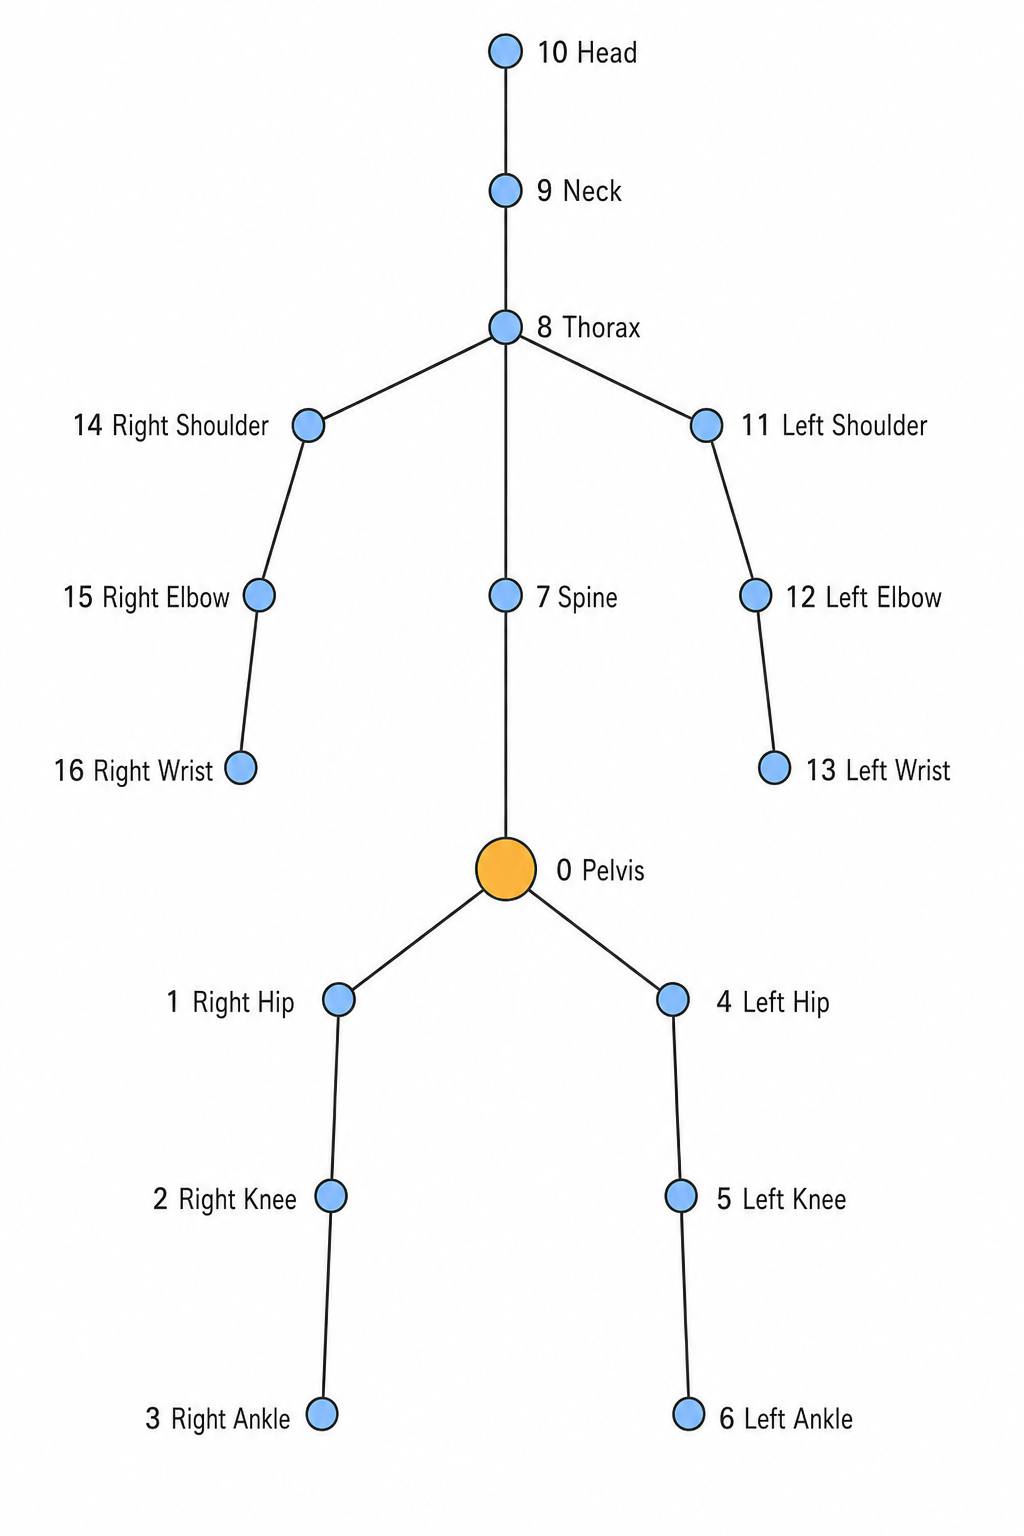
\includegraphics[width=0.85\textwidth]{figures/kinematic_tree.pdf}
\fbox{\parbox[c][6cm][c]{0.85\textwidth}{\centering\textit{[Kinematic-tree figure:
  insert \texttt{figures/kinematic\_tree.pdf}. The 17-joint Human3.6M skeleton as a
  rooted tree, pelvis (0) as root, 16 parent-child bones; each joint labelled with its
  index and name.]}}}
\caption[The Human3.6M skeleton as a rooted kinematic tree.]{The 17-joint
  Human3.6M skeleton, represented as a rooted kinematic tree $G=(V,E)$
  with the pelvis (joint 0) as root and 16 parent-child bone edges. The
  naive scan order used by default in Section~\ref{sec:method-bistssm}
  simply follows the numerical joint index shown in each node, ignoring
  this tree structure entirely.}
\label{fig:kinematic-tree}
\end{figure}

\section{Preliminaries: State Space Models}
\label{sec:method-prelim}

Before the architecture is described, this section states the state space
formulation the backbone is built on, following the line of work reviewed in
Section~\ref{sec:lit-ssm-foundations}. A continuous-time linear state space
model maps an input signal $u(t)$ to an output $y(t)$ through a hidden state
$h(t) \in \mathbb{R}^{N}$,
\begin{equation}
\dot{h}(t) = A h(t) + B u(t), \qquad y(t) = C h(t),
\label{eq:ssm-continuous}
\end{equation}
where $A \in \mathbb{R}^{N \times N}$ governs how the state evolves and $B$,
$C$ map the input in and the state out. To run on a discrete sequence, the
system is discretized with a step size $\Delta$ using a zero-order hold,
\begin{equation}
\bar{A} = \exp(\Delta A), \qquad
\bar{B} = (\Delta A)^{-1}\big(\exp(\Delta A) - I\big)\, \Delta B,
\label{eq:ssm-discretize}
\end{equation}
which turns Equation~\ref{eq:ssm-continuous} into the recurrence applied along
the sequence,
\begin{equation}
h_k = \bar{A} h_{k-1} + \bar{B} u_k, \qquad y_k = C h_k .
\label{eq:ssm-recurrence}
\end{equation}
S4 \cite{gu2021s4} made this practical at scale with a structured
parameterization of $A$, and S5 \cite{smith2022s5} recast it as a single
multi-input, multi-output system computed by a parallel scan. In all of these
the parameters $\bar{A}$, $\bar{B}$, $C$, and $\Delta$ are fixed for the whole
sequence.

Mamba \cite{gu2023mamba} makes the model \emph{selective}: it computes $B$,
$C$, and $\Delta$ as functions of the current input token, so the system can
decide at each position what to write into the state and what to read out.
This input dependence is what lets a state space model match attention on
content-dependent reasoning while keeping a recurrence that is linear in
sequence length. The resulting scan is evaluated with a hardware-aware
parallel algorithm that avoids writing the full sequence of hidden states to
slow memory. KinecMamba uses a diagonal $A$ with a hidden state of size
$N=16$, and applies this selective formulation as the core of its state space
layer (Section~\ref{sec:method-bistssm}).

\section{Architecture Overview}
\label{sec:method-architecture}

KinecMamba is a dual-stack, Mamba-based architecture that
processes the input 2D keypoint sequence in four stages: token embedding,
a stack of bidirectional spatio-temporal state space blocks, and an
output head. All internal token representations use a fixed channel width
of $C=64$.

\textbf{Token embedding.} The input $X \in \mathbb{R}^{B \times T \times J
\times 2}$ is first mapped to $C$-dimensional tokens by the Spatial Token
Embedding (STE), then augmented with temporal position information by the
Temporal Token Embedding (TTE), producing $Z^{(0)} \in \mathbb{R}^{B
\times T \times J \times C}$. Both embedding stages are detailed in
Section~\ref{sec:method-embedding}.

\textbf{Backbone.} $Z^{(0)}$ is then processed by 10 macro-stages. Each
macro-stage applies a Spatial-oriented BiSTSSMBlock followed by a
Temporal-oriented BiSTSSMBlock, for 20 BiSTSSMBlock instances in total.
Every BiSTSSMBlock, regardless of its spatial or temporal designation,
shares the identical internal residual structure detailed in
Section~\ref{sec:method-block} and is built around the same BiSTSSM layer,
a four-directional cross-scan selective state space layer (detailed in
Section~\ref{sec:method-bistssm}) operating over the full $T \times J$
grid of token embeddings. Each BiSTSSMBlock contains approximately 63,000
parameters (approximately 46,000 in the state space path and 17,000 in
the feed-forward path), giving a 20-block backbone of approximately 1.26
million parameters. The token embeddings and the linear output head add
only a small further amount, so the complete model contains on the order
of 1.26 million parameters, the figure reported for it in
Chapter~\ref{ch:results}.

\textbf{Output head.} After the final BiSTSSMBlock, the resulting
representation $Z^{(20)} \in \mathbb{R}^{B \times T \times J \times C}$ is
projected to 3D joint coordinates by an output head consisting of layer
normalization followed by a linear projection, $C \rightarrow 3$,
producing the predicted 3D pose sequence $\hat{Y} \in \mathbb{R}^{B \times
T \times J \times 3}$ defined in Section~\ref{sec:method-problem}.

In summary, the end-to-end shape flow, also shown in
Figure~\ref{fig:architecture-pipeline}, is:
\[
X \in \mathbb{R}^{B,T,J,2}
\;\xrightarrow{\text{STE, TTE}}\;
Z^{(0)} \in \mathbb{R}^{B,T,J,C}
\;\xrightarrow{\text{20} \times \text{BiSTSSMBlock}}\;
Z^{(20)} \in \mathbb{R}^{B,T,J,C}
\;\xrightarrow{\text{output head}}\;
\hat{Y} \in \mathbb{R}^{B,T,J,3}.
\]

\begin{figure}[t]
\centering
% Architecture figure: place the rendered image at figures/architecture.pdf and
% uncomment the \includegraphics line below (remove the placeholder box). The image
% is generated from figure_prompts.md (Figure 1).
% 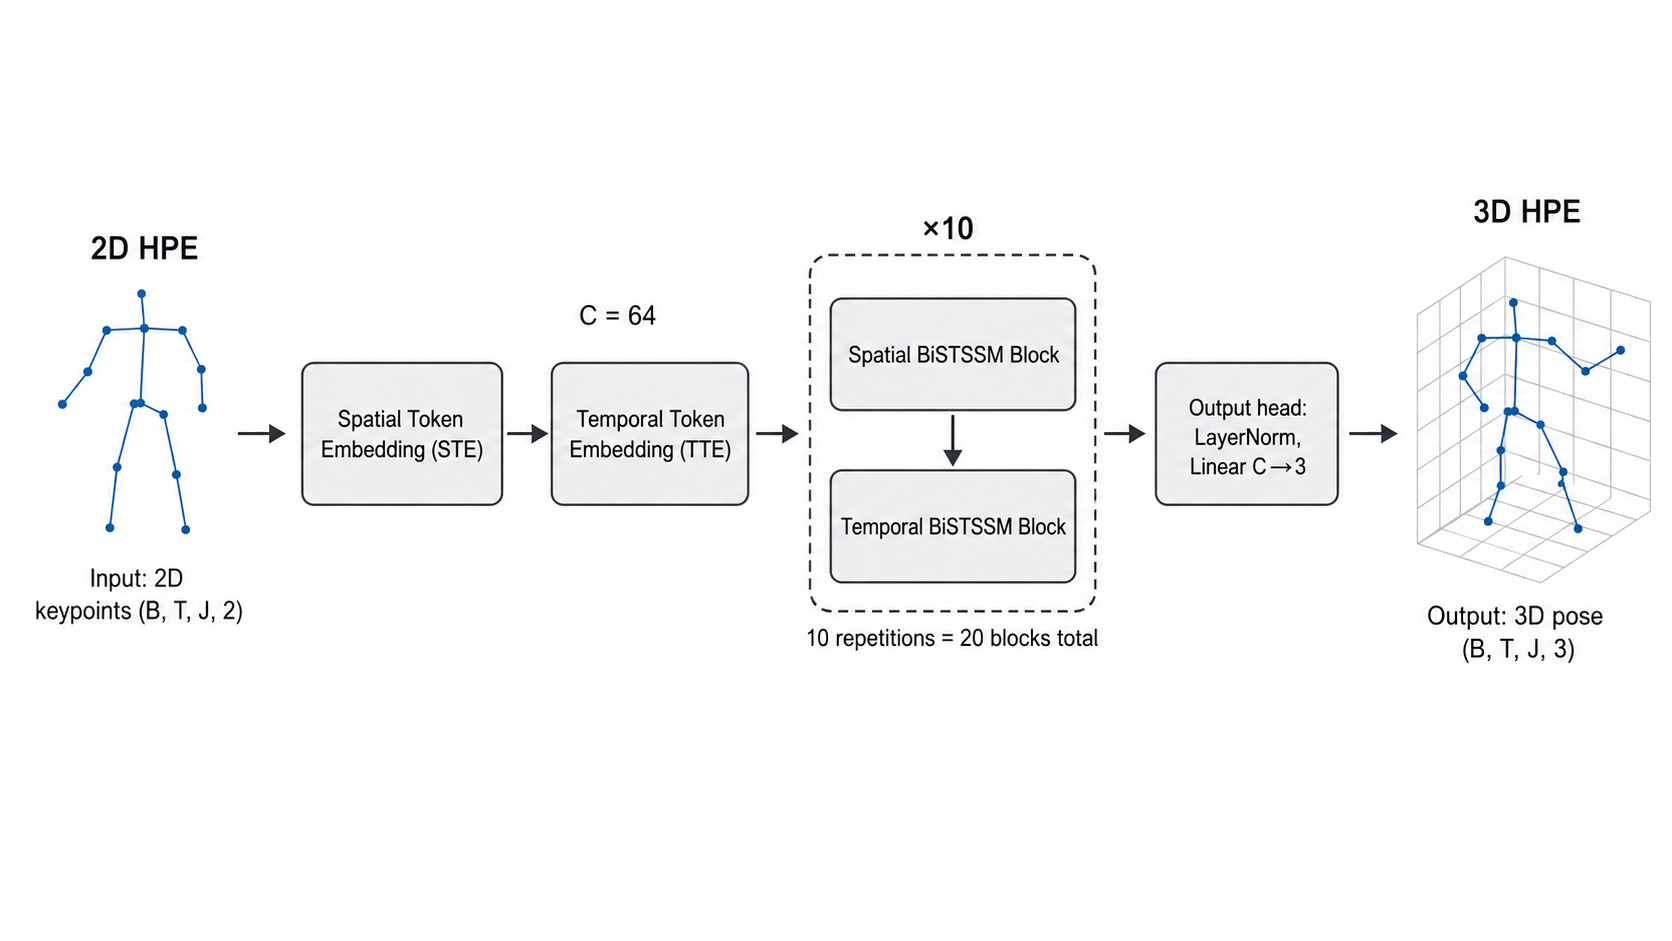
\includegraphics[width=\textwidth]{figures/architecture.pdf}
\fbox{\parbox[c][5.5cm][c]{0.92\textwidth}{\centering\textit{[Architecture
  diagram: insert \texttt{figures/architecture.pdf}. 2D-pose input
  $(B,T,J,2)$ $\rightarrow$ STE $\rightarrow$ TTE $\rightarrow$ $\times$10
  Spatial/Temporal BiSTSSM backbone (20 blocks) $\rightarrow$ output head
  (LayerNorm, Linear $C{\to}3$) $\rightarrow$ 3D-pose output $(B,T,J,3)$.]}}}
\caption[End-to-end architecture pipeline.]{End-to-end architecture
  pipeline. The input 2D keypoint sequence is embedded by the STE and TTE
  (Section~\ref{sec:method-embedding}), processed by 10 repetitions of a
  Spatial BiSTSSMBlock followed by a Temporal BiSTSSMBlock (20 blocks
  total, Section~\ref{sec:method-block}), and projected to the output 3D
  pose sequence by the output head.}
\label{fig:architecture-pipeline}
\end{figure}

\section{Spatial and Temporal Token Embedding}
\label{sec:method-embedding}

The raw input $X \in \mathbb{R}^{B \times T \times J \times 2}$ is
converted into $C$-dimensional tokens in two stages, each of which
combines a learned projection with a learned positional embedding along a
different axis.

\textbf{Spatial Token Embedding (STE).} The batch and frame dimensions are
first merged, treating every $(batch, frame)$ pair as an independent set
of $J$ joints: $X \in \mathbb{R}^{B,T,J,2} \rightarrow \mathbb{R}^{BT,J,2}$.
A shared linear layer, $\mathrm{Linear}(2 \rightarrow C)$, projects each
joint's raw 2D coordinate into the $C$-dimensional token space. A learned
spatial positional embedding $P_{\mathrm{sp}} \in \mathbb{R}^{1,J,C}$,
broadcast across the merged $BT$ dimension, is then added, so that each of
the $J$ token positions carries a fixed, learnable identity independent of
the coordinate values placed into it. The result is reshaped back to
$\mathbb{R}^{B,T,J,C}$.

\textbf{Temporal Token Embedding (TTE).} The batch and joint dimensions
are then merged instead, treating every $(batch, joint)$ pair as an
independent length-$T$ time series: $\mathbb{R}^{B,T,J,C} \rightarrow
\mathbb{R}^{BJ,T,C}$. A learned temporal positional embedding
$P_{\mathrm{te}} \in \mathbb{R}^{1,T,C}$, broadcast across the merged $BJ$
dimension, is added directly (no additional linear projection is needed
at this stage, since the tokens are already $C$-dimensional), giving each
of the $T$ frame positions a fixed, learnable identity. The result is
reshaped back to $\mathbb{R}^{B,T,J,C}$, producing $Z^{(0)}$, the input to
the first BiSTSSMBlock.

Because $P_{\mathrm{sp}}$ is indexed by joint position and added before
any scan-order permutation is applied, each token's positional identity
travels with it through any subsequent reordering of the joint axis. This
is what allows the scan order over the joint axis (the naive index order,
or the breadth-first kinematic-tree order introduced in
Section~\ref{sec:method-bfs}) to be changed without altering what
information the network has available to identify which physical joint
each token corresponds to.

\section{The Bidirectional Spatio-Temporal State Space Block}
\label{sec:method-block}

Every BiSTSSMBlock, whether spatial- or temporal-oriented, is a pre-norm
residual block containing two sub-layers: the BiSTSSM layer itself
(Section~\ref{sec:method-bistssm}) and a position-wise feed-forward
network, each wrapped in a residual connection preceded by layer
normalization. Given an input token grid $z \in \mathbb{R}^{B,T,J,C}$, the
block computes:
\begin{align}
z' &= z + \mathrm{DropPath}\big(\mathrm{BiSTSSM}(\mathrm{LayerNorm}(z))\big), \\
z'' &= z' + \mathrm{DropPath}\big(\mathrm{MLP}(\mathrm{LayerNorm}(z'))\big),
\end{align}
where $\mathrm{DropPath}$ is stochastic depth. During training, the
entire sub-layer's contribution is randomly zeroed with some probability
and the residual connection alone is passed through, which regularizes the
network without altering its structure at inference time. The
feed-forward network expands and then contracts the channel dimension,
\begin{equation}
\mathrm{MLP}(u) = \mathrm{Linear}_{128 \rightarrow 64}\big(\mathrm{GELU}(\mathrm{Linear}_{64 \rightarrow 128}(u))\big),
\end{equation}
applied identically and independently to every token in the $T \times J$
grid. This pre-norm residual design mirrors the block structure used
throughout the Transformer- and SSM-based literature reviewed in
Chapter~\ref{ch:literature-review}; what distinguishes the block proposed
here is the internal design of the BiSTSSM layer itself, detailed next.

\section{The BiSTSSM Layer: Cross-Scan Selective State Space Modeling}
\label{sec:method-bistssm}

The BiSTSSM layer is the component within each BiSTSSMBlock
(Section~\ref{sec:method-block}) responsible for modeling dependencies
across the $T \times J$ grid of token embeddings. It operates in six
steps: a four-directional cross-scan, an input projection, a depthwise
convolution, a selective state space model applied per direction, a
cross-merge, and an output projection. Figure~\ref{fig:bistssm-layer}
summarizes this pipeline.

\begin{figure}[t]
\centering
% BiSTSSM-layer figure: place the rendered image at figures/bistssm_layer.pdf and
% uncomment the \includegraphics line below (remove the placeholder box). The image is
% generated from figure_prompts.md (Figure 3, BiSTSSM layer internals).
% 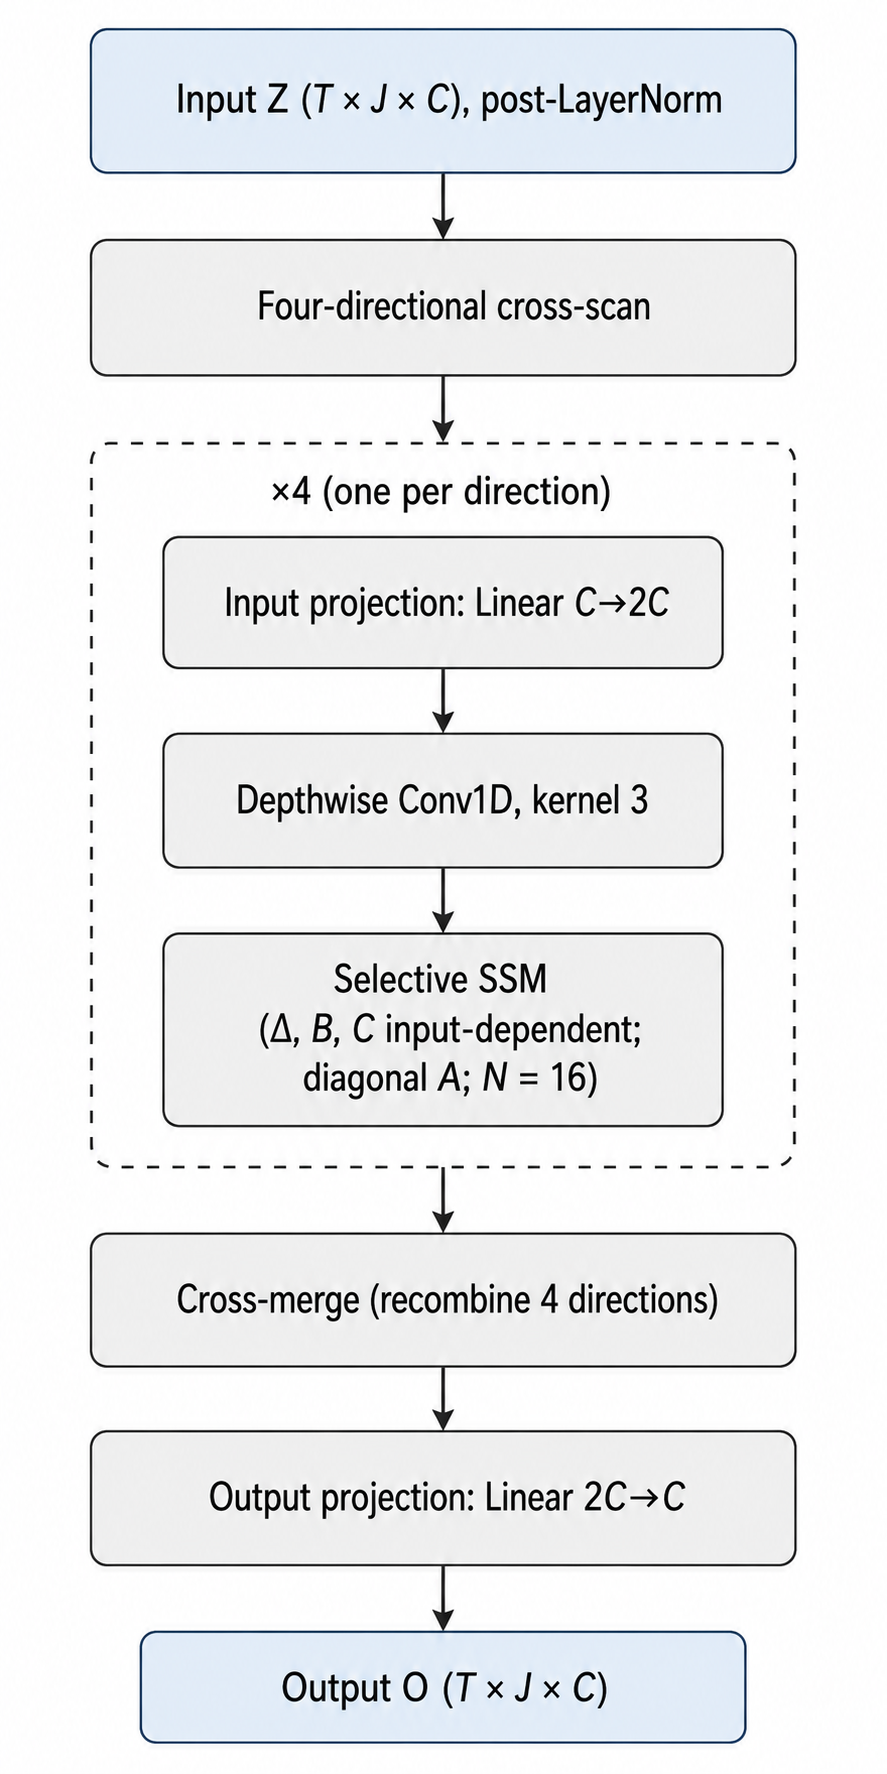
\includegraphics[width=0.6\textwidth]{figures/bistssm_layer.pdf}
\fbox{\parbox[c][6cm][c]{0.6\textwidth}{\centering\textit{[BiSTSSM-layer figure: insert
  \texttt{figures/bistssm\_layer.pdf}. Vertical pipeline: input $Z$ (post-LayerNorm)
  $\rightarrow$ four-directional cross-scan $\rightarrow$ $\times$4 (input projection
  $C{\to}2C$, depthwise Conv1D k=3, selective SSM with $N{=}16$) $\rightarrow$ cross-merge
  $\rightarrow$ output projection $2C{\to}C$ $\rightarrow$ output $O$.]}}}
\caption[The BiSTSSM layer.]{The BiSTSSM layer: the $T\times J$ token
  grid is unfolded into four directional sequences, each independently
  projected, convolved, and processed by a selective state space model,
  then recombined by the cross-merge step and projected back to the
  model's working width $C$.}
\label{fig:bistssm-layer}
\end{figure}

\textbf{Four-directional cross-scan.} A selective state space model, as
reviewed in Section~\ref{sec:lit-ssm-foundations}, processes a strictly
one-dimensional sequence, whereas the layer's input is a 2D grid of $T
\times J$ tokens. Following the cross-scan strategy introduced for
non-causal visual data by VMamba \cite{liu2024vmamba} and the
bidirectional scanning of Vision Mamba \cite{zhu2024visionmamba}, the
layer unfolds this grid into four separate 1D sequences from two natural
flattenings, each read in both directions. The first flattening is
frame-major, sweeping all joints within a frame before advancing to the next
frame; the second is joint-major, sweeping all frames for a joint before
advancing to the next joint. Reading each flattening forward and then
backward gives the four sequences. Each is processed by an independent
instance of the remaining steps below, so that every token is eventually
informed by grid neighbors reached from all four traversal directions, not
only those preceding it in a single fixed order.

\textbf{Input projection and local convolution.} Each of the four
directional sequences, with tokens of width $C=64$, is first projected to
an expanded width of $2C=128$ by a linear layer, giving the selective SSM
step below more representational capacity to work with than the model's
residual-stream width. A depthwise 1D convolution with kernel size 3 is
then applied along the sequence dimension, independently per channel,
giving each token a small amount of local context (its immediate
neighbors in the current scan order) before the global, recurrent
computation of the state space model.

\textbf{Selective state space model.} Each of the four length-$L$
sequences (where $L=TJ$) is then processed by a selective state space model,
the formulation set out in Section~\ref{sec:method-prelim}
\cite{gu2023mamba}. The post-convolution sequence supplies the input tokens
$u_k$; the hidden state has dimension $N=16$; the state matrix $A$ is diagonal
with negative entries, which keeps the recurrence stable; and $B_k$, $C_k$,
and the step size $\Delta_k$ are computed per token, so the layer decides at
each scan position what to write into and read out of the state. The
recurrence of Equation~\ref{eq:ssm-recurrence} is evaluated with the
hardware-aware parallel scan of Mamba \cite{gu2023mamba}, which never
materializes the full sequence of hidden states in slow memory.

\textbf{Cross-merge and output projection.} Once all four directional
sequences have been processed, each is reshaped back into the $T \times J$
grid layout and the four resulting grids are combined into a single
$2C$-dimensional grid representation in the cross-merge step, mirroring
the merge stage of VMamba's cross-scan \cite{liu2024vmamba}. A final linear
layer projects this merged representation from $2C=128$ back down to
$C=64$, matching the residual-stream width used by the surrounding
BiSTSSMBlock (Section~\ref{sec:method-block}).

\section{Breadth-First Search Kinematic-Tree Scan Order}
\label{sec:method-bfs}

The row-major and column-major flattenings underlying the cross-scan
described in Section~\ref{sec:method-bistssm} require an explicit order
over the $J$ joints along the spatial axis of the grid. By default, this
order is simply the joint's numerical index, $[0, 1, \ldots, 16]$, which
carries no relationship to the skeleton's actual anatomical structure: for
example, under this order, joint 3 (Right Ankle) and joint 4 (Left Hip)
are scan-adjacent despite being on opposite sides of the body and far
apart in the kinematic tree $G$ defined in
Section~\ref{sec:method-problem}. As discussed in
Section~\ref{sec:lit-skeleton-ordering}, this thesis instead orders the
joints by a breadth-first search (BFS) traversal of $G$, which visits
joints in order of their distance from the root and so keeps each joint
close in the sequence to its parent and to the other joints at its depth,
rather than to arbitrary joints elsewhere in the skeleton.

\textbf{BFS traversal.} Algorithm~\ref{alg:bfs-scan} formalizes the
traversal. Starting from the root joint (the pelvis, joint 0), the
algorithm visits joints in order of non-decreasing graph distance from the
root, breaking ties by visiting a node's children in
ascending original joint-index order. This tie-breaking rule ensures the
resulting order $\pi$ is fixed and reproducible for a given kinematic tree
$G$, in contrast to the learned Group and
Joint Scan strategies of \cite{nguyen2025skeletonmamba} reviewed in
Section~\ref{sec:lit-ssm-pose}.

\renewcommand{\algorithmicrequire}{\textbf{Input:}}
\renewcommand{\algorithmicensure}{\textbf{Output:}}
\renewcommand{\algorithmicforall}{\textbf{for each}}
\begin{algorithm}
\caption{Breadth-First Search Kinematic-Tree Scan Order}
\label{alg:bfs-scan}
\begin{algorithmic}
  \REQUIRE $G=(V,E)$: kinematic tree over joints $V=\{0,\ldots,J-1\}$
    (Section~\ref{sec:method-problem}), rooted at joint $r=0$ (pelvis)
  \ENSURE $\pi$: an ordered list of joint indices, a permutation of $V$
  \STATE $\pi \gets$ empty list; $Q \gets$ empty queue
  \STATE mark $r$ as visited; enqueue $r$ onto $Q$
  \WHILE{$Q$ is not empty}
    \STATE $v \gets$ dequeue from $Q$
    \STATE append $v$ to $\pi$
    \FORALL{children $c$ of $v$ in $E$, in ascending index order}
      \IF{$c$ is not visited}
        \STATE mark $c$ as visited; enqueue $c$ onto $Q$
      \ENDIF
    \ENDFOR
  \ENDWHILE
  \STATE \textbf{return} $\pi$
\end{algorithmic}
\end{algorithm}

Applied to the Human3.6M kinematic tree of Section~\ref{sec:method-problem},
Algorithm~\ref{alg:bfs-scan} produces the fixed order
\[
\pi = [\,0,\ 1,\ 4,\ 7,\ 2,\ 5,\ 8,\ 3,\ 6,\ 9,\ 11,\ 14,\ 10,\ 12,\ 15,\ 13,\ 16\,],
\]
that is, Pelvis; Right Hip, Left Hip, Spine; Right Knee, Left Knee, Thorax;
Right Ankle, Left Ankle, Neck, Left Shoulder, Right Shoulder; Head, Left
Elbow, Right Elbow; Left Wrist, Right Wrist. The traversal visits the
skeleton level by level outward from the pelvis, exactly as motivated in
Section~\ref{sec:lit-skeleton-ordering}. Figure~\ref{fig:scan-order-comparison}
contrasts this order directly against the naive index order it replaces:
under the naive order, anatomically distant joints (e.g.\ Right Ankle and
Left Hip) are scan-adjacent, whereas under the proposed BFS order,
scan-adjacent joints are also kinematically close.

\begin{figure}[t]
\centering
% Scan-order figure: place the rendered image at figures/scan_order.pdf and uncomment
% the \includegraphics line below (remove the placeholder box). The image is generated
% from figure_prompts.md (Figure 4, naive vs BFS scan order).
% \includegraphics[width=\textwidth]{figures/scan_order.pdf}
\fbox{\parbox[c][3.5cm][c]{0.95\textwidth}{\centering\textit{[Scan-order figure: insert
  \texttt{figures/scan\_order.pdf}. Two strips of 17 joint cells: a top ``naive index
  order'' strip (0..16) and a bottom ``BFS kinematic order'' strip
  (0,1,4,7,2,5,8,3,6,9,11,14,10,12,15,13,16), showing that the BFS order keeps
  kinematically close joints adjacent.]}}}
\caption[Naive vs.\ BFS kinematic-tree scan order.]{The 17 joints
  (abbreviated names, subscript = joint index, as defined in
  Figure~\ref{fig:kinematic-tree}) under the naive index order used by
  default (top) versus the proposed breadth-first kinematic-tree order
  $\pi$ (bottom). The BFS order visits joints level by level outward from
  the pelvis, so joints at the same depth in the kinematic tree become
  adjacent (e.g.\ the two hips and the spine root, all direct children of
  the pelvis) and every joint stays close to its parent, whereas the naive
  order interleaves joints from unrelated parts of the skeleton.}
\label{fig:scan-order-comparison}
\end{figure}

\textbf{Permute-before-scan, inverse-permute-after-merge.} Let $Z \in
\mathbb{R}^{B,T,J,C}$ be a BiSTSSMBlock's input to the BiSTSSM layer, with
joints indexed in the original order established by the spatial
positional embedding (Section~\ref{sec:method-embedding}). Before the
cross-scan of Section~\ref{sec:method-bistssm} is applied, $Z$ is reindexed
along its joint axis according to $\pi$,
\begin{equation}
Z_\pi[:,:,i,:] = Z[:,:,\pi(i),:], \qquad i = 0, \ldots, J-1,
\end{equation}
Because this reindexing is applied to the joint axis of $Z$ before either
flattening is formed, all four directional scans, in both the frame-major
and joint-major flattenings of Section~\ref{sec:method-bistssm}, traverse
joints in kinematic-tree BFS order rather than raw index order. After the selective state space model
and cross-merge produce an output $O_\pi \in \mathbb{R}^{B,T,J,C}$, still
in BFS order, the inverse permutation $\pi^{-1}$ is applied to restore the
original joint indexing,
\begin{equation}
O[:,:,\pi(i),:] = O_\pi[:,:,i,:], \qquad i = 0, \ldots, J-1,
\end{equation}
before $O$ is returned as $\mathrm{BiSTSSM}(\cdot)$ in the residual
equation of Section~\ref{sec:method-block}. This inverse permutation is
essential: without it, the residual addition $z + \mathrm{BiSTSSM}(z)$
would add each joint's input token to a \emph{different} joint's output
token, and the fixed, joint-indexed spatial positional embedding of
Section~\ref{sec:method-embedding} would no longer correspond to the
correct joint after the first block.

Because $\pi$ is derived once from the fixed kinematic tree $G$ and
applied identically to every BiSTSSMBlock, this scan order adds only a
fixed gather/scatter operation, distinguishing it from the auxiliary
topology-fusion modules and learned scan groupings reviewed in
Section~\ref{sec:lit-ssm-pose}.

\section{Computational Complexity}
\label{sec:method-complexity}

The efficiency claim behind KinecMamba can be stated directly. Let $L = TJ$
be the number of spatio-temporal tokens the BiSTSSM layer processes. The
selective state space scan of Section~\ref{sec:method-bistssm} visits each
token once and, at each step, updates a hidden state of fixed size $N$, so
its cost grows as $\mathcal{O}(L N C)$, that is, linearly in $L$ for fixed
$N$ and channel width $C$. The four directional scans and the depthwise
convolution add only constant factors. Full spatio-temporal self-attention,
by contrast, forms an $L \times L$ score matrix and therefore costs
$\mathcal{O}(L^{2} C)$, quadratic in $L$. This is the gap identified as
Problem~1 in Section~\ref{sec:intro-problem-statement}: at a sequence length
of $L = 243 \times 17 = 4131$ tokens, the quadratic term is what forces
attention-based lifters into a trade-off between temporal window and
compute, and it is what the state space backbone removes.

The breadth-first scan order does not change this analysis. It is a fixed
permutation of the $J$ joints along one axis, applied as a gather before the
scan and a scatter after the merge (Section~\ref{sec:method-bfs}), so it costs
$\mathcal{O}(J)$ per layer. KinecMamba therefore keeps the linear-time
behaviour of its backbone while changing only the order in which joints enter
the scan.

\section{Loss Function}
\label{sec:method-loss}

The network is trained with a multi-term loss. Four terms are standard in
prior 3D HPE work \cite{zhang2022mixste, zhu2023motionbert,
mehraban2024motionagformer} and target per-frame joint accuracy, robustness
to scale ambiguity, temporal velocity, and prediction smoothness. Two
further terms are anatomy-aware bone-length losses that pair with the BFS
kinematic scan of Section~\ref{sec:method-bfs}, supervising the lengths and
temporal consistency of the skeleton's bones. Let $\hat{Y}, Y \in
\mathbb{R}^{B,T,J,3}$ denote the predicted and ground-truth 3D pose sequences
defined in Section~\ref{sec:method-problem}.

\textbf{Joint position loss.} The primary supervision signal is the mean
per-joint position error (MPJPE), the mean Euclidean distance between
predicted and ground-truth joint positions:
\begin{equation}
\mathcal{L}_{3d} = \frac{1}{BTJ} \sum_{b,t,j} \big\lVert \hat{Y}_{b,t,j} - Y_{b,t,j} \big\rVert_2 .
\end{equation}

\textbf{Scale-invariant joint position loss.} Because monocular depth
estimates are subject to a global scale ambiguity, a second term evaluates
accuracy after removing any consistent scale error. For each sample, the
least-squares optimal scale factor aligning the prediction to the ground
truth,
\begin{equation}
s^{*} = \frac{\sum_{t,j} \hat{Y}_{t,j} \cdot Y_{t,j}}{\sum_{t,j} \hat{Y}_{t,j} \cdot \hat{Y}_{t,j}},
\end{equation}
is computed and applied before measuring MPJPE:
\begin{equation}
\mathcal{L}_{3d\text{-}scale} = \frac{1}{BTJ} \sum_{b,t,j} \big\lVert s^{*} \hat{Y}_{b,t,j} - Y_{b,t,j} \big\rVert_2 .
\end{equation}

\textbf{Velocity loss.} To encourage temporally coherent motion, a third
term compares frame-to-frame joint velocities of the prediction and the
ground truth, $\Delta \hat{Y}_{t} = \hat{Y}_{t+1} - \hat{Y}_{t}$ and
$\Delta Y_{t} = Y_{t+1} - Y_{t}$:
\begin{equation}
\mathcal{L}_{3d\text{-}velocity} = \frac{1}{B(T-1)J} \sum_{b,t,j} \big\lVert \Delta \hat{Y}_{b,t,j} - \Delta Y_{b,t,j} \big\rVert_2 .
\end{equation}

\textbf{Temporal smoothness loss.} A fourth term regularizes the
prediction's own frame-to-frame smoothness directly, independent of the
ground-truth velocity, via a per-joint weighted quadratic penalty on
consecutive-frame differences:
\begin{equation}
\mathcal{L}_{diff} = \frac{1}{B(T-1)J} \sum_{b,t,j} w_j \big\lVert \Delta \hat{Y}_{b,t,j} \big\rVert_2^{2},
\end{equation}
where $w_j$ is a fixed, per-joint weighting coefficient.

\textbf{Bone-length loss.} The length of each bone is fixed by the body and
should not change with pose or over time, so two anatomy-aware terms
supervise the skeleton's bones. Let $E$ be the set of 16 parent-child bones
of the kinematic tree $G$ (Section~\ref{sec:method-problem}), and let
$\ell_e(\hat{Y}_{t})$ denote the Euclidean length of bone $e$ in the
predicted pose at frame $t$. The first term matches predicted bone lengths to
the ground truth,
\begin{equation}
\mathcal{L}_{bone} = \frac{1}{BT|E|} \sum_{b,t,e} \big| \ell_e(\hat{Y}_{b,t}) - \ell_e(Y_{b,t}) \big|,
\end{equation}
and the second penalizes the temporal variance of each predicted bone length,
\begin{equation}
\mathcal{L}_{bvar} = \frac{1}{B|E|} \sum_{b,e} \mathrm{Var}_{t}\big[ \ell_e(\hat{Y}_{b,t}) \big].
\end{equation}
Both terms act on the same 16 bones the BFS scan of
Section~\ref{sec:method-bfs} traverses, so the training objective and the
scan order reinforce the same skeletal structure.

\textbf{Combined objective.} The total training loss is a weighted sum of
the six terms:
\begin{equation}
\mathcal{L} = \lambda_{3d}\, \mathcal{L}_{3d} + \lambda_{scale}\, \mathcal{L}_{3d\text{-}scale} + \lambda_{vel}\, \mathcal{L}_{3d\text{-}velocity} + \lambda_{diff}\, \mathcal{L}_{diff} + \lambda_{bone}\, \mathcal{L}_{bone} + \lambda_{bvar}\, \mathcal{L}_{bvar},
\end{equation}
with $\lambda_{3d} = 1.0$, $\lambda_{scale} = 0.5$, $\lambda_{vel} = 20.0$,
$\lambda_{diff} = 0.5$, $\lambda_{bone} = 0.5$, and $\lambda_{bvar} = 1.0$.
The comparatively large weight on $\mathcal{L}_{3d\text{-}velocity}$ reflects
its role as the primary driver of temporal consistency between predicted and
ground-truth motion, while the bone-length terms keep the predicted skeleton
anatomically consistent.

\section{Summary}
\label{sec:method-summary}

This chapter presented KinecMamba, a dual-stack, Mamba-based architecture for
monocular 3D human pose estimation. Section~\ref{sec:method-problem}
formalized the input/output representation and the skeleton's kinematic
tree, and Section~\ref{sec:method-embedding} projects the input 2D
keypoint sequence into a fixed-width token representation. A stack of 20
bidirectional spatio-temporal state space
blocks (Section~\ref{sec:method-block}), each built around a
four-directional cross-scan selective state space layer
(Section~\ref{sec:method-bistssm}), models spatial and temporal
dependencies with linear complexity in sequence length, consistent with
the efficiency motivation established in Chapter~\ref{ch:literature-review}.
The chapter's central contribution, the breadth-first search kinematic-tree
scan order (Section~\ref{sec:method-bfs}), replaces the naive joint-index
order otherwise used by this cross-scan with a traversal
derived directly from the skeleton's own parent-child hierarchy, closing
the research gap identified in Section~\ref{sec:lit-summary-gap}.
Section~\ref{sec:method-loss}
defined the loss function, which combines standard position, scale,
velocity, and smoothness terms with two anatomy-aware bone-length terms that
reinforce the same skeletal structure as the BFS scan.
Chapter~\ref{ch:results} evaluates this architecture empirically, reporting
accuracy and computational efficiency on the Human3.6M and MPI-INF-3DHP
benchmarks against the baselines identified in
Chapter~\ref{ch:literature-review}, and presenting ablation studies that
isolate the specific contribution of the BFS kinematic-tree scan order.

\FloatBarrier


\setlength{\footskip}{8mm}

\chapter{Experimental Results}
\label{ch:results}

\section{Overview}
\label{sec:results-overview}

Chapter~\ref{ch:methodology} presented a dual-stack, Mamba-based
architecture for monocular 3D human pose estimation, centered on a
breadth-first search (BFS) kinematic-tree scan order
(Section~\ref{sec:method-bfs}) intended to close the research gap
identified in Section~\ref{sec:lit-summary-gap}. This chapter reports the
empirical evaluation of that architecture.

Section~\ref{sec:results-protocol} describes the benchmark datasets and
the evaluation metrics used throughout this chapter.
Section~\ref{sec:results-implementation} summarizes the implementation
configuration. Section~\ref{sec:results-h36m} sets out the main comparison
of this thesis, placing KinecMamba against established baselines
on Human3.6M that span the Transformer and state-space families.
Section~\ref{sec:results-mpiinf3dhp} and Section~\ref{sec:results-ablation}
cover the MPI-INF-3DHP benchmark, whose cross-dataset evaluation is in
progress, and the scan-order ablation study motivated in
Section~\ref{sec:intro-objectives}, which is set out as future work. The main
Human3.6M evaluation is reported in full.
Section~\ref{sec:results-summary} closes the chapter.

\section{Datasets and Evaluation Protocol}
\label{sec:results-protocol}

\textbf{Human3.6M} \cite{ionescu2014human36m} is the primary benchmark used
in this thesis. It consists of 3.6 million video frames of 11 professional
actors performing 15 everyday actions, captured by four synchronized
cameras in a controlled studio, with 3D ground-truth annotations obtained
via a marker-based motion capture system. Following the standard protocol
established by the baselines reviewed in Chapter~\ref{ch:literature-review}
\cite{pavllo2019videopose3d, zheng2021poseformer, zhang2022mixste}, subjects
S1, S5, S6, S7, and S8 are used for training and subjects S9 and S11 for
testing. The 17-joint skeleton format used throughout is the one defined
in Section~\ref{sec:method-problem}.

\textbf{MPI-INF-3DHP} \cite{mehta2017mpiinf3dhp} is used as a secondary,
cross-dataset benchmark. It includes a greater diversity of actions,
subjects, and both indoor and outdoor recording conditions than
Human3.6M, and is commonly used to assess how well a model generalizes
beyond a single controlled capture setup.

\textbf{Evaluation metrics.} Two standard metrics are used, both computed
on the root-relative 3D pose representation defined in
Section~\ref{sec:method-problem}. The first, Protocol~1 (P1), is the mean
per-joint position error (MPJPE) already defined as the primary training
loss term in Section~\ref{sec:method-loss},
\begin{equation}
\text{MPJPE} = \frac{1}{TJ} \sum_{t,j} \big\lVert \hat{Y}_{t,j} - Y_{t,j} \big\rVert_2 ,
\end{equation}
averaged here over the test set rather than a training batch. The second,
Protocol~2 (P-MPJPE), first applies a per-frame rigid Procrustes alignment
(denoted $\mathrm{Proc}(\cdot)$: a least-squares optimal rotation,
translation, and scale, unlike the scale-only correction used by the
training-time $\mathcal{L}_{3d\text{-}scale}$ term in
Section~\ref{sec:method-loss}) between the predicted and ground-truth
pose before computing MPJPE:
\begin{equation}
\text{P-MPJPE} = \frac{1}{TJ} \sum_{t,j} \big\lVert \mathrm{Proc}(\hat{Y}_{t}, Y_{t})_{j} - Y_{t,j} \big\rVert_2 .
\end{equation}
Both metrics are reported in millimeters. Unless otherwise noted, all P1
and P2 figures in this chapter, for the proposed method and for every
baseline alike, correspond to the ``detected 2D'' input setting, in which 2D
keypoints are obtained from an off-the-shelf 2D pose detector rather than
ground-truth annotations, consistent with the standard evaluation
convention in the literature reviewed in Chapter~\ref{ch:literature-review}.

\section{Implementation Details}
\label{sec:results-implementation}

The evaluated model follows exactly the architecture and training
objective specified in Chapter~\ref{ch:methodology}: an input window of
$T=243$ frames over $J=17$ joints, a token width of $C=64$, 20
BiSTSSMBlock instances (Section~\ref{sec:method-architecture}), a
selective state space hidden dimension of $N=16$
(Section~\ref{sec:method-bistssm}), the breadth-first search
kinematic-tree scan order $\pi$ (Section~\ref{sec:method-bfs}), and the
six-term loss function with $\lambda_{3d}=1.0$, $\lambda_{scale}=0.5$,
$\lambda_{vel}=20.0$, $\lambda_{diff}=0.5$, $\lambda_{bone}=0.5$, and
$\lambda_{bvar}=1.0$ (Section~\ref{sec:method-loss}).

The model is trained with the AdamW optimizer (weight decay 0.01) under a
cosine learning-rate schedule, using an effective batch size of 32 reached
through gradient accumulation, with horizontal-flip augmentation applied to
the 2D input sequences. Input 2D keypoints are the Stacked Hourglass
detections distributed with the Human3.6M benchmark. Training and evaluation
are carried out on a single GPU.

\section{Comparison with the State of the Art on Human3.6M}
\label{sec:results-h36m}

Table~\ref{tab:h36m-sota} places KinecMamba alongside
representative recent baselines from Chapter~\ref{ch:literature-review},
using each baseline's officially reported P1/P2 figures under the protocol
defined in Section~\ref{sec:results-protocol}. To keep the comparison against
current methods, the table lists baselines at or below PoseMamba's reported
error; older and weaker entries are omitted. KinecMamba reaches an MPJPE (P1)
of 41.55mm and a P-MPJPE (P2) of 34.52mm on the S9 and S11 test split, at a
parameter budget of roughly 1.26M.

\begin{table}[t]
\centering
\caption[Comparison with the state of the art on Human3.6M.]{Comparison
  with the state of the art on Human3.6M under the detected-2D input
  setting. $T$: number of input frames. Params/MACs are as officially
  reported by each method; ``n/r'' denotes a value not reported in the
  cited source. The proposed method is shown in bold.
  P1: MPJPE (mm). P2: P-MPJPE (mm).}
\label{tab:h36m-sota}
\resizebox{\textwidth}{!}{%
\begin{tabular}{l l c c c c c}
\hline
Method & Venue & $T$ & Params (M) & MACs (G) & P1 $\downarrow$ & P2 $\downarrow$ \\
\hline
\multicolumn{7}{l}{\textit{Transformer-based}} \\
MixSTE \cite{zhang2022mixste}             & CVPR'22  & 243 & 33.6 & 139.0 & 40.9  & 32.6 \\
STCFormer \cite{tang2023stcformer}        & CVPR'23  & 243 & 4.7  & 19.6  & 41.0  & 32.0 \\
MotionBERT \cite{zhu2023motionbert}       & ICCV'23  & 243 & 42.3 & 174.8 & 39.2  & 32.9 \\
MotionAGFormer-L \cite{mehraban2024motionagformer} & WACV'24 & 243 & 19.0 & 78.3 & 38.4 & 32.5 \\
\hline
\multicolumn{7}{l}{\textit{State-space-based}} \\
Pose Magic \cite{zhang2024posemagic}      & 2024     & 243 & 14.4 & 40.6  & 37.5  & 31.8 \\
PoseMamba-S \cite{huang2025posemamba}     & AAAI'25  & 243 & 0.9  & 3.6   & 41.8  & 35.0 \\
SasMamba \cite{cui2025sasmamba}           & WACV'26  & 243 & 0.64 & 1.3   & 41.48 & 34.84 \\
\hline
\textbf{KinecMamba (ours)} & This work & 243 & \textbf{1.26} & n/r & \textbf{41.55} & \textbf{34.52} \\
\hline
\end{tabular}%
}
\end{table}

At approximately 1.26M parameters, KinecMamba sits in the same
efficiency tier as the smallest baselines in Table~\ref{tab:h36m-sota},
alongside PoseMamba-S (0.9M) and SasMamba (0.64M), rather
than the large-model tier of MotionBERT, MotionAGFormer-L, or Pose Magic.
Because the architectural contribution of this thesis is a change of scan
order rather than of model capacity, the closest point of comparison is
PoseMamba-S in the same tier. At a comparable parameter budget, KinecMamba's
MPJPE (41.55mm) and P-MPJPE (34.52mm) are marginally below those of
PoseMamba-S (41.8mm / 35.0mm), and in the same range as the other compact
state-space model, SasMamba (41.48mm P1 / 34.84mm P2), slightly higher on P1
and slightly lower on P2. The larger baselines in the table (MotionBERT,
MotionAGFormer-L, Pose Magic) reach lower MPJPE, but at roughly ten to thirty
times the parameter count, placing them in a different capacity tier.
Section~\ref{sec:results-ablation} describes the
scan-order ablation that would attribute the difference from PoseMamba-S to
the BFS kinematic-tree scan itself rather than to other differences in
training configuration. Figure~\ref{fig:results-plot} plots accuracy against
model size for all methods in the table.

\begin{figure}[t]
\centering
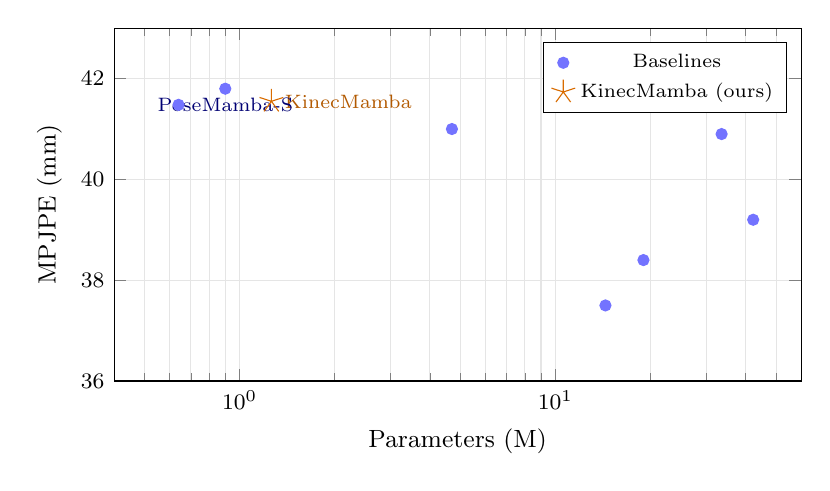
\begin{tikzpicture}
\begin{axis}[
  width=0.85\textwidth, height=0.5\textwidth,
  xlabel={Parameters (M)}, ylabel={MPJPE (mm)},
  xmode=log, log basis x=10,
  xmin=0.4, xmax=60, ymin=36, ymax=43,
  grid=both, grid style={gray!20},
  tick label style={font=\footnotesize},
  label style={font=\small},
  legend style={font=\scriptsize, at={(0.98,0.96)}, anchor=north east},
  nodes near coords style={font=\scriptsize},
]
% Baseline points: (params in M, MPJPE mm) from Table~\ref{tab:h36m-sota}
\addplot[only marks, mark=*, mark size=2pt, color=blue!55] coordinates {
  (33.6,40.9) (4.7,41.0) (42.3,39.2) (19.0,38.4) (14.4,37.5)
  (0.9,41.8) (0.64,41.48)
};
\addlegendentry{Baselines}
% KinecMamba (ours): measured Human3.6M result from Table~\ref{tab:h36m-sota}
\addplot[only marks, mark=star, mark size=4.5pt, color=orange!85!black] coordinates {
  (1.26,41.55)
};
\addlegendentry{KinecMamba (ours)}
\node[anchor=west, font=\scriptsize, color=orange!70!black] at (axis cs:1.26,41.55) {\,KinecMamba};
\node[anchor=north, font=\scriptsize, color=blue!45!black] at (axis cs:0.9,41.8) {PoseMamba-S};
\end{axis}
\end{tikzpicture}
\caption[Accuracy versus model size on Human3.6M.]{Accuracy (MPJPE, lower is
  better) against model size for the methods of Table~\ref{tab:h36m-sota} on
  Human3.6M. KinecMamba (1.26M parameters, 41.55mm) sits in the compact
  state-space tier, with error marginally below its closest baseline
  PoseMamba-S (0.9M, 41.8mm) at a comparable parameter budget.}
\label{fig:results-plot}
\end{figure}

\section{Results on MPI-INF-3DHP}
\label{sec:results-mpiinf3dhp}

Section~\ref{sec:intro-objectives} committed this thesis to evaluating
KinecMamba on MPI-INF-3DHP \cite{mehta2017mpiinf3dhp} in
addition to Human3.6M, in order to assess generalization beyond a single
controlled capture setup, following the same protocol used by prior
state-space pose estimators
\cite{tang2023stcformer, huang2025posemamba, cui2025sasmamba}.

The cross-dataset evaluation on MPI-INF-3DHP is currently in progress. The
data pipeline for this benchmark is prepared and the model is being evaluated
under the protocol used by the prior state-space estimators above; the MPJPE,
PCK, and AUC results will be reported in this section once the run completes.
The main empirical claim of this thesis rests on the Human3.6M comparison in
Section~\ref{sec:results-h36m}.

\section{Ablation Study}
\label{sec:results-ablation}

A comparison on Human3.6M alone (Section~\ref{sec:results-h36m}) cannot
by itself attribute any difference from PoseMamba-S to a single cause.
Such a difference could follow from the BFS kinematic-tree scan order
(Section~\ref{sec:method-bfs}), from incidental differences in training
configuration, or from a combination of the two.
Objective 4 in Section~\ref{sec:intro-objectives} committed this thesis to
an ablation study designed to resolve this question directly, holding the
architecture (Sections~\ref{sec:method-block}--\ref{sec:method-bistssm})
and training configuration (Section~\ref{sec:results-implementation})
fixed and varying only the spatial scan order applied within the
BiSTSSM layer, comparing three conditions:
\begin{enumerate}
  \item the naive index order $[0, 1, \ldots, 16]$ (the default, illustrated
    in Figure~\ref{fig:kinematic-tree});
  \item the proposed breadth-first search kinematic-tree order $\pi$
    (Section~\ref{sec:method-bfs}); and
  \item a learned scan order in the style of the Group and Joint Scan
    strategies of \cite{nguyen2025skeletonmamba}, as the representative
    learned-scan alternative reviewed in Section~\ref{sec:lit-ssm-pose}.
\end{enumerate}

This controlled scan-order ablation is left as future work. The Human3.6M
result in Section~\ref{sec:results-h36m} compares KinecMamba to PoseMamba-S,
its closest baseline in architecture and parameter budget, but that single
comparison cannot on its own isolate the BFS kinematic-tree scan order from
incidental differences in training configuration. Running the three
scan-order conditions above under one fixed architecture and training setup,
so that only $\pi$ varies, is the direct way to make that attribution, and is
listed among the recommendations in
Section~\ref{sec:conclusion-recommendations}.

\section{Summary}
\label{sec:results-summary}

This chapter set out the evaluation of the architecture presented in
Chapter~\ref{ch:methodology} on Human3.6M, positioning it at roughly
1.26M parameters within the same efficiency tier as the smallest
baselines reviewed in Chapter~\ref{ch:literature-review}
(Section~\ref{sec:results-h36m}). On that benchmark KinecMamba reaches
41.55mm MPJPE and 34.52mm P-MPJPE, marginally below its closest baseline
PoseMamba-S (41.8mm / 35.0mm) at a comparable parameter budget and in the
same range as the compact state-space model SasMamba. The cross-dataset
evaluation on MPI-INF-3DHP (Section~\ref{sec:results-mpiinf3dhp}) is in
progress, and the scan-order ablation that would isolate the contribution of
the BFS kinematic-tree scan (Section~\ref{sec:results-ablation}) is set out as
future work.
Chapter~\ref{ch:conclusion} summarizes the contributions of this thesis in
light of these results, discusses their limitations, and outlines the work
that remains.

\FloatBarrier


\setlength{\footskip}{8mm}

\chapter{Conclusion and Recommendations}
\label{ch:conclusion}

\section{Conclusion}
\label{sec:conclusion-conclusion}

This thesis addressed a specific gap identified in
Chapter~\ref{ch:literature-review}: existing Transformer-based methods
for monocular 3D human pose estimation scale quadratically with sequence
length, and existing state-space-based alternatives, while linear in
sequence length, order the skeleton's joints either by an anatomically
arbitrary fixed index or by a learned scan grouping, rather than by the
skeleton's own kinematic structure (Section~\ref{sec:lit-summary-gap}).

Chapter~\ref{ch:methodology} presented KinecMamba, a dual-stack, Mamba-based
architecture for this task, built around a four-directional cross-scan
selective state space layer (Section~\ref{sec:method-bistssm}), and
introduced this thesis's central contribution: a breadth-first search
kinematic-tree scan order (Section~\ref{sec:method-bfs}) that replaces
the naive joint-index order with a traversal derived directly from the
skeleton's parent-child hierarchy, together with an anatomy-aware
bone-length loss that reinforces the same skeletal structure.
Chapter~\ref{ch:results} set out the evaluation of KinecMamba on Human3.6M,
which places it in the same efficiency tier as the smallest baselines
compared against, namely PoseMamba-S and SasMamba. At roughly 1.26M
parameters it reaches 41.55mm MPJPE and 34.52mm P-MPJPE. Measured against
PoseMamba-S, the closest baseline in both architecture and parameter budget
(41.8mm / 35.0mm), this is an improvement on both metrics without an increase
in model capacity, and it is competitive with the other compact state-space
model, SasMamba. The cross-dataset evaluation on MPI-INF-3DHP and the
scan-order ablation were left as future work.

The Human3.6M result supports the thesis's motivating hypothesis, that a
scan order derived from the skeleton's kinematic tree can improve a
state-space-based pose estimator without increasing model capacity: at a
comparable parameter budget KinecMamba lowers both MPJPE and P-MPJPE relative
to PoseMamba-S. This support should be read with one caveat. As discussed in
Section~\ref{sec:results-ablation}, a comparison on Human3.6M alone does not
by itself isolate the BFS scan order as the specific cause of the difference
from PoseMamba-S, as opposed to incidental differences in training
configuration. The scan-order ablation designed to make that attribution
directly, and the MPI-INF-3DHP cross-dataset evaluation committed to in
Section~\ref{sec:intro-objectives}, were left as future work
(Sections~\ref{sec:results-mpiinf3dhp}~and~\ref{sec:results-ablation}). A
claim that the BFS kinematic-tree scan order specifically, rather than the
architecture or training configuration as a whole, drives the improvement
should therefore be treated as provisional pending that ablation.

\section{Recommendations}
\label{sec:conclusion-recommendations}

The following work is recommended to complete and extend this thesis:

\begin{enumerate}
  \item \textbf{Complete the pending evaluations.} The scan-order
    ablation study (Section~\ref{sec:results-ablation}) and the
    MPI-INF-3DHP evaluation (Section~\ref{sec:results-mpiinf3dhp}) should
    be finished and reported, and the training hyperparameters and
    hardware configuration omitted from Section~\ref{sec:results-implementation}
    should be finalized and documented, so that the results in this
    thesis are fully reproducible.

  \item \textbf{Extend the ablation beyond a single model size and sequence
    length.} Because the Human3.6M comparison in Section~\ref{sec:results-h36m}
    is conducted at a single, small parameter budget and a fixed 243-frame
    window, it remains untested whether the benefit of the BFS kinematic-tree
    scan persists, grows, or diminishes at larger model capacities such as
    those of PoseMamba-L or MotionAGFormer-L, or at longer input windows,
    where a state space scan's implicit memory can begin to decay
    \cite{zhang2024kmm}.

  \item \textbf{Explore hybrid fixed/learned scan orders.} The BFS scan
    order is fixed by the skeleton's kinematic tree
    (Section~\ref{sec:method-bfs}), while methods such as
    \cite{nguyen2025skeletonmamba} learn scan groupings from data. A
    natural extension is a hybrid approach that initializes a learned scan
    from the BFS kinematic-tree order rather than from a random or
    index-based starting point, potentially combining the interpretability
    of a kinematically-grounded order with the flexibility of a learned
    one.

  \item \textbf{Test generalization beyond the evaluated scope.} As noted
    in Section~\ref{sec:intro-limitations}, this thesis is restricted to
    single-person, monocular, fixed-topology input. Extending the BFS
    kinematic-tree scan to multi-person scenes, to skeletal topologies
    other than the Human3.6M 17-joint format (e.g.\ hand or face
    keypoints), or to in-the-wild video without ground-truth 3D annotation
    would test how specific the method's benefit is to the evaluated
    setting.

  \item \textbf{Report qualitative and per-action results.} Aggregate
    MPJPE and P-MPJPE (Section~\ref{sec:results-h36m}) do not indicate
    which actions or motion types benefit most from the proposed scan
    order. A per-action breakdown and qualitative visualization of
    predicted versus ground-truth motion sequences would clarify where the
    architectural contribution of this thesis helps most.
\end{enumerate}

\FloatBarrier



% NEED TO CHANGE THE SECTION NUMBER FOR REFERENCES ACCORDINGLY.
\renewcommand{\bibname}{REFERENCES}
\addcontentsline{toc}{chapter}{6 \hskip 3.55em References}

%\bibliographystyle{apacite}
\bibliographystyle{IEEEtran}  % For IEEE format {apacite} --> {IEEEtran}
\bibliography{references}

% COMMENT THE LINES ABOUT APPENDICS OUT IF YOU DO NOT HAVE THIS SECTION.

%%%%%%%%%%%%%%%%%%%%%%%%%%%%%%%%%%%%%%%%%%%%%%%%%%%%%%%%%%%%%%%%%%%
%                                                                 %
%                            APPENDICES                           %
%                                                                 %
%%%%%%%%%%%%%%%%%%%%%%%%%%%%%%%%%%%%%%%%%%%%%%%%%%%%%%%%%%%%%%%%%%%
\newpage\pagestyle{plain}
\theappendix

% NEED TO CHANGE THE SECTION NUMBER FOR REFERENCES ACCORDINGLY.
\addcontentsline{toc}{chapter}{7 \hskip 3.55em Appendices}

\setlength{\footskip}{8mm}

\renewcommand{\thefigure}{A.\arabic{figure}}
\renewcommand{\thetable}{A.\arabic{table}}

\begin{center}
{\large \bf Appendix A\\ \vskip 1em Kinematic Tree and BFS Scan Order\\ \vskip 1em}
\vskip 1em
\end{center}

\FloatBarrier

\singlespace

This appendix lists the 17-joint Human3.6M skeleton used throughout the thesis
(Section~\ref{sec:method-problem}) and the breadth-first search (BFS) scan order
derived from it (Section~\ref{sec:method-bfs}).

\vskip 1em
{\bf Joints.} The 17 joints are indexed as: 0 pelvis, 1 right hip, 2 right knee,
3 right ankle, 4 left hip, 5 left knee, 6 left ankle, 7 spine, 8 thorax, 9 neck,
10 head, 11 left shoulder, 12 left elbow, 13 left wrist, 14 right shoulder,
15 right elbow, 16 right wrist.

\vskip 1em
{\bf Bones (kinematic-tree edges).} The 16 parent-child bones, rooted at the pelvis
(joint 0), grouped by chain:

\begin{itemize}
  \item Right leg: $0\rightarrow1\rightarrow2\rightarrow3$
  \item Left leg: $0\rightarrow4\rightarrow5\rightarrow6$
  \item Spine and head: $0\rightarrow7\rightarrow8\rightarrow9\rightarrow10$
  \item Left arm: $8\rightarrow11\rightarrow12\rightarrow13$
  \item Right arm: $8\rightarrow14\rightarrow15\rightarrow16$
\end{itemize}

\vskip 1em
{\bf BFS scan order.} Visiting joints outward from the pelvis, level by level, and
breaking ties by ascending joint index, gives the order
\[
\pi = [\,0,\ 1,\ 4,\ 7,\ 2,\ 5,\ 8,\ 3,\ 6,\ 9,\ 11,\ 14,\ 10,\ 12,\ 15,\ 13,\ 16\,].
\]
The BiSTSSM layer reindexes the joint axis by $\pi$ before the spatial scan and applies
the inverse permutation after the cross-merge, as described in
Section~\ref{sec:method-bfs}.

\FloatBarrier


\end{document}

